\documentclass[11pt,a4paper]{ctexart}
\usepackage[margin=2.45cm,marginparwidth=1.35cm,marginparsep=0.18cm]{geometry}
\usepackage{amsmath,amssymb,amsthm}
\usepackage{graphicx}
\usepackage{float}
\usepackage[font=small,labelsep=quad]{caption}
\usepackage{fancyhdr}
\usepackage{enumitem}
\usepackage[colorlinks=false,hidelinks]{hyperref}
\linespread{1.28}
\setlength{\parindent}{2em}
\pagestyle{fancy}\fancyhf{}\fancyfoot[C]{\thepage}\renewcommand{\headrulewidth}{0pt}
\newcommand{\SourcePage}[1]{\marginpar{\raggedright\footnotesize 原文 p.#1}}
\newcommand{\SrcRange}[2]{\ifnum#1=#2\marginpar{\raggedright\footnotesize 原文 p.#1}\else\marginpar{\raggedright\footnotesize 原文 pp.#1--#2}\fi}
\newcommand{\TN}[1]{\footnote{译注：#1}}
\allowdisplaybreaks
\begin{document}
\begin{center}
{\LARGE\bfseries 从物理视角看 $K$-理论}\\[6pt]
{\large K-Theory from a Physical Perspective}\\[6pt]
Gregory Moore\\[2pt]
{\small arXiv:hep-th/0304018}\\[8pt]
{\small 中文译注本 v2.0 重制版（2026-11-14）}
\end{center}
\vspace{0.6em}
\noindent{\small\bfseries 重制说明.} 本册按《数学文献翻译纪律》v2.0 重制：以原文为底本逐段核对，公式、图、文献与页锚点均回查原文；旧版（Markdown→DOCX→PDF）已隔离。页边注「原文 pp.N--M」标出该节对应的原文页码范围；文献保留英文条目与原文编号。凡属译者补充而原文无者，均注明依据或标「译者按（无外部依据）」。
\vspace{1em}

\providecommand{\tightlist}{\setlength{\itemsep}{0pt}\setlength{\parskip}{0pt}}
本文是一篇综述性文章，旨在阐明关于 \(D\)-膜 \(K\)-理论分类的一种物理观点。我们把边界共形场论之间重整化群流的想法，与反常相消、\(D\)-膜瞬子效应等时空概念结合起来。我们通过描述特殊酉群 \(SU(N)\) 的扭曲 K-理论来展示这一观点。

\SrcRange{2}{2}
\section{引言}\label{ux5f15ux8a00}

本文是一篇综述性文章，致力于解释 \(D\)-膜 \(K\)-理论分类的若干方面。我们的目标是以与（Minasian and Moore 1997; Witten 1998）的讨论相补充的方式来处理这一主题。对后一类进路的综述包括（Olsen and Szabo 1999; Witten 2001; Freed 2002; Szabo 2002）。我们预设的读者，是熟悉共形场论与 \(K\)-理论、并对（非共形）量子场论这一更广阔领域怀有一定兴趣的数学家。

本文的安排如下：第 2 节先回顾拓扑场论层面上 \(D\)-膜与 K-理论的关系。接着在第 3 节转向共形场论中的 \(D\)-膜。我们将倡导一种观点，即把二维共形场论视为更大的二维量子场论空间中的元素。``D-膜''被等同于带边二维流形上的共形量子场论。从这一视角看，\(D\)-膜的拓扑分类，就是带边二维流形上那些仅通过其边界条件破坏共形不变性的理论的构型空间的连通分支的分类。

在第 4 节我们将转向用于构造弦论的共形场论。在这种情况下，\(D\)-膜的分类有一个时空视角。我们将给出一种基于反常相消与``瞬子效应''的 \(D\)-膜分类观点，它与 Atiyah-Hirzebruch 谱序列密切相关。

在第 5 节我们考察一个具体的例子，即 WZW 模型中的膜，并说明如何运用第 3、4 节所解释的进路，对 \(SU(N)\) 的扭曲 K-理论获得直观的理解。这一图像与 M. Hopkins 的一个严格计算美妙地吻合。

我们要在开头就提醒读者：在这篇篇幅不大的综述中，我们只打算对若干想法给出一个粗线条的概述。我们既不打算给出一个细致而严格的数学理论，也不打算对该主题作全面的综述。

\SrcRange{3}{6}
\section{二维拓扑场论中的膜}\label{ux4e8cux7ef4ux62d3ux6251ux573aux8bbaux4e2dux7684ux819c}

\(D\)-膜与 K-理论的关系，可以在二维（2D）拓扑场论这一极其简单的情形中被非常清楚地展示出来。这一讨论是与 Graeme Segal 合作发展的（Moore and Segal，未发表）。

我们将按照 Segal 在本文集中的贡献所采取的方式来理解``场论''。它是一个从几何范畴到某个线性范畴的函子。在二维拓扑场论的简单情形中，几何范畴的对象是不交圆的并，态射是对象之间有向配边的微分同胚类。目标范畴是向量空间与线性变换的范畴。回忆一下：给定一个闭弦的二维拓扑场论，等价于给定一个交换的、有限维的 Frobenius 代数 \({\mathcal C}\)。例如，其代数结构来自图 1。

\begin{figure}[tbp]
\centering
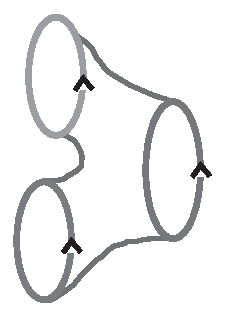
\includegraphics[width=0.28\textwidth,height=0.22\textheight,keepaspectratio]{fig01.pdf}
\caption{三孔曲面对应于 Frobenius 代数的基本乘法。}
\end{figure}


现在让我们把几何范畴扩大，使之同时包含开弦与闭弦。此时既有入射/出射的圆，也有入射/出射的区间，而态射是带有两类边界的曲面：入射/出射边界，以及由入射/出射区间的端点扫出的``自由边界''。这些自由边界必须用``边界条件''来标记，而在目前，它们只是一些标记 \(a,b,\dots\)。

\begin{figure}[tbp]
\centering
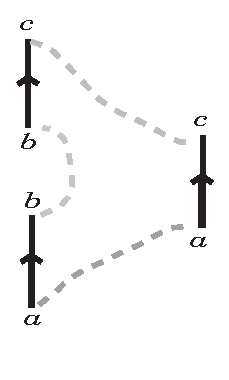
\includegraphics[width=0.28\textwidth,height=0.22\textheight,keepaspectratio]{fig02.pdf}
\caption{定义开弦的非阿贝尔 Frobenius 代数的乘法。}
\end{figure}


因为我们有一个函子，所以对任意一对边界条件我们都联系一个向量空间（``一个态空间''）\({\mathcal H}_{ab}\)。此外，还存在一个相容的双线性乘积系统

\[{\mathcal H}_{ab}\otimes {\mathcal H}_{bc} \rightarrow {\mathcal H}_{ac}\]

它由图 2 定义。这就引出我们的关键问题：\emph{什么样的边界条件与 \({\mathcal C}\) 相容？} ``相容''指的是与曲面的``缝合''（sewing）或``粘合''（gluing）相容；更确切地说，我们希望得到一个良定义的函子。因此，正如式上式定义了一个结合交换代数结构于 \({\mathcal C}\) 之上，图 2 在 \(a=b=c\) 的情形下在 \({\mathcal H}_{aa}\) 上定义了一个（不必交换的）代数结构。此外，\({\mathcal H}_{aa}\) 是一个 Frobenius 代数。其次，还有进一步把开弦结构与闭弦结构联系起来的缝合条件。例如，我们要求图 3 与图 4 所定义的算子相等，这一条件有时被称为``Cardy 条件''。

\begin{figure}[tbp]
\centering
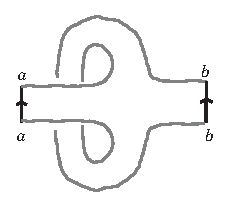
\includegraphics[width=0.28\textwidth,height=0.22\textheight,keepaspectratio]{fig03.pdf}
\caption{在开弦通道中，该曲面在非交换 Frobenius 代数上定义了一个自然算子 $\pi: {\mathcal H}_{aa} \to {\mathcal H}_{bb}$。}
\end{figure}


\begin{figure}[tbp]
\centering
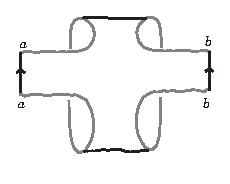
\includegraphics[width=0.28\textwidth,height=0.22\textheight,keepaspectratio]{fig04.pdf}
\caption{在闭弦通道中，该曲面定义了开-闭与闭-开跃迁的复合 $\iota_{c-o}\iota_{o-c}: {\mathcal H}_{aa} \to {\mathcal H}_{bb}$，它通过中心分解。}
\end{figure}


正如 Segal 早些时候所指出的（Segal 1999），对公式上式的正确解释是：边界条件是一个加法范畴中的对象 \(a,b,\dots\)，并满足

\[{\mathcal H}_{ab} = {\mathrm Mor}(a,b).\]

因此，我们应当问：缝合约束对边界条件的范畴意味着什么？这个问题实际上包含两部分：第一，缝合的相容性等价于目标范畴上的某种代数结构。一旦我们确定了这一结构，就可以要求对这种结构的实例进行分类。问题的第一部分已被完全解答：开/闭缝合条件最早由 Cardy 与 Lewellen 分析（Cardy and Lewellen 1991; Lewellen 1992），而所得的代数结构在（Moore and Segal，未发表; Lazaroiu 2001）中被描述。结果如下：

\textbf{命题} 给定一个开-闭二维有向拓扑场论，等价于给定

\begin{enumerate}
\def\labelenumi{\arabic{enumi}.}
\item
  一个交换 Frobenius 代数 \({\mathcal C}\)。
\item
  对每个边界条件 \(a\)，一个 Frobenius 代数 \({\mathcal H}_{aa}\)。
\item
  一个同态 \(\iota_a: {\mathcal C} \to Z({\mathcal H}_{aa})\)（其中 \(Z({\mathcal H}_{aa})\) 是中心），满足 \(\iota_a(1) = 1\)，并且若 \(\iota^a\) 是 \(\iota_a\) 的伴随，则
\end{enumerate}

\[\pi_b^{~a} = \iota_b \iota^a.\]

这里 \(\pi_b^{~a}: {\mathcal H}_{aa} \to {\mathcal H}_{bb}\) 是由图 3 所描述的态射，它完全由开弦数据决定。当 \({\mathcal H}_{ab}\) 为非零向量空间时，它是一个 Morita 等价双模，而 \(\pi_b^{~a}\) 可写成 \(\pi_b^{~a}(\psi) = \sum \psi^\mu \psi \psi_\mu\)，其中 \(\psi_\mu\) 是 \({\mathcal H}_{ab}\) 的一组基，\(\psi^\mu\) 是 \({\mathcal H}_{ba}\) 的对偶基。更不变量地，

\[\theta_b(\pi_b^{~a}(\psi) \mathrm{ch}i) = {{\mathrm{Tr}}}_{{\mathcal H}_{ab}}\left( L(\psi) R(\mathrm{ch}i)\right)\]

其中 \(\theta_b\) 是 \({\mathcal H}_{bb}\) 上的迹，\(L(\psi),R(\mathrm{ch}i)\) 分别是 \({\mathcal H}_{aa}\)、\({\mathcal H}_{bb}\) 在 \({\mathcal H}_{ab}\) 上的左表示与右表示。

第二步，即找出这类结构的所有实例，在（Moore and Segal，未发表）中就 \({\mathcal C}\) 为半单 Frobenius 代数的情形作了分析。答案非常干净利落：

\textbf{定理 1} 设 \({\mathcal C}\) 是半单的。则边界条件范畴中对象的同构类集合为

\[K^0({\mathrm Spec}({\mathcal C}))= K_0({\mathcal C}) .\]

当 \({\mathcal C}\) \emph{不是}半单的时候，上述结构也有重要的实例，例如拓扑的 \(A\)-型与 \(B\)-型扭曲 \({\mathcal N}=2\) 超对称 sigma 模型。据我们所知，非半单 \({\mathcal C}\) 情形下的实例分类仍是一个未解决的问题。

即便在这一初等的框架之中，也存在有趣而不平凡的推广。当一个二维闭拓扑场论具有对称性 \(G\) 时，就可以对它作``规范化''（gauging）。配边范畴通过考虑主 \(G\)-丛的配边而得到扩充。此时闭拓扑场论对应于一个``Turaev 代数''（Turaev 1999; Moore and Segal，未发表）的选取，它是 Frobenius 代数的一种 \(G\)-等变扩充；在半单情形，它由一个``时空''（由离散的点集构成，对应于代数的幂等元）、一个``伸缩子''（dilaton，编码 Frobenius 代数在各幂等元上的迹）以及一个``\(B\)-场''来刻画。此时我们有

\textbf{定理 2} 对于时空为 \(X\)、``\(B\)-场''为 \([b]\in H^2_G(X;C^*)\) 的 \(G\)-等变开-闭理论，其边界条件范畴中对象的同构类，与 \(G\)-等变、\(b\)-扭曲的 \(K\)-理论类所构成的 K-群 \(K_{G,b}(X)\) 一一对应。

当然，这些结果都非常初等。我觉得它们迷人之处恰恰在于它们\emph{是}如此原始：它们只依赖拓扑缝合条件与一点点代数，而 K-理论却不可避免地浮现出来。

关于有理共形场论中膜的范畴论式分类，已有更为精细的进路，见 文献。

\SrcRange{7}{15}
\section{K-理论与重整化群}\label{k-ux7406ux8bbaux4e0eux91cdux6574ux5316ux7fa4}

\subsection{在边界上破坏共形不变性}\label{ux5728ux8fb9ux754cux4e0aux7834ux574fux5171ux5f62ux4e0dux53d8ux6027}

现在让我们考虑一个困难得多的问题：在完整的共形场论（CFT）中，D-膜的拓扑分类。这立刻引出这样一个问题：我们所说的``D-膜''究竟指什么。也许最有成效的观点是：D-膜是二维 CFT \({\mathcal C}\) 中保持共形对称性的\emph{局部}边界条件。尽管关于 D-膜的文献浩如烟海，人们实际研究过的那些具体膜其实只是所有可能情形中极小的一部分。

研究 D-膜分类的一条途径，是考虑定义在带边界曲面上的二维量子场论（QFT）所构成的空间，这些场论\emph{并不}共形，而只是通过其边界条件破坏共形不变性。形式地说，存在一个空间 \({\mathcal B}\)，由与固定``体''CFT \({\mathcal C}\) 相容的这类边界 QFT 组成。\({\mathcal B}\) 的切空间就是边界上局部算子构成的空间，因为局部算子 \({\mathcal O}\) 可以用来把曲面 \(\Sigma\) 上的作用量形变：

\[S_{\mathrm worldsheet} =S_{\mathrm bulk CFT}  + \int_{\partial \Sigma}  ds {\mathcal O}\]

这里 \(ds\) 是线元。注意，这一项一般会引入显式的度规依赖，从而在边界上破坏共形不变性。

作为我们所设想情形的一个简单例子，考虑一个无质量标量场 \(x^\mu:\Sigma\to \mathbb{R}^n\)，其作用量为

\[S_{\mathrm worldsheet} =\int_\Sigma \partial x^\mu \bar{\partial} x^\mu  + \int_{\partial \Sigma}  ds T\bigl(x^\mu(\tau)\bigr)\]

其中 \(T(x^\mu)\) 是 \(\mathbb{R}^n\) 上的``任意函数''，\(\tau\) 是 \(\partial \Sigma\) 上的坐标。于是，上式中的边界相互作用可以展开为

\[{\mathcal O}  = T(x) + A_\mu(x)\frac{dx^\mu}{d \tau} + B_{\mu}(x) \frac{d^2 x^\mu}{d\tau^2} +
C_{\mu\nu}(x) \frac{dx^\mu}{d \tau}  \frac{dx^\nu}{d \tau}   + \cdots\]

系数 \(T(x), A_\mu(x),\dots\) 被看作靶空间 \(\mathbb{R}^n\) 上的时空场。\TN{G. Segal 向我指出，边界 CFT 切空间的恰当表述自然会用到 jet 理论。}

我们预期可以给 \({\mathcal B}\) 赋予一种拓扑，使得重整化群流（见下文）是这个空间上的连续演化。在这种拓扑下，\({\mathcal B}\) 是不连通的空间。核心的想法是：这个空间的\emph{连通分支}由某种 \(K\)-理论来分类。例如，若该共形场论是超对称的，并且具有非线性 \(\sigma\) 模型意义上的靶空间解释，我们预期 \({\mathcal B}\) 的连通分支对应于靶空间 \(X\) 的 K-理论

\[\pi_0({\mathcal B}) = K(X).\]

注记：

\begin{itemize}
\item
  \begin{enumerate}
  \def\labelenumi{\arabic{enumi}.}
  \tightlist
  \item
    在上式中，我们刻意对 K-理论的确切形式（例如是 \(K\)，还是 \(KO,KR,K_\pm\) 等等）含糊其辞。这取决于在构造该二维场论时所作的一组离散选择。
  \end{enumerate}
\item
  2. 从这个观点看，世界面上存在某种超对称的重要性是清楚的。正如下一节的例子所表明的，把 \({\mathcal O}\) 取为单位算子所对应的 RG 流总是流向``没有边界''的平庸不动点。因此，除非单位算子能够被投影掉，\({\mathcal B}\) 中不可能有有意思的道路连通分支。用时空的语言说，我们必须消去``零动量快子''。
\item
  3. 人们可能会问：当 CFT 没有明显的靶空间解释时，什么取代上式？一个可能的答案是：应当为开弦顶点算子代数定义某种代数 K-理论。近来在更深入地理解 Witten 的 Chern-Simons 开弦场论方面已有许多进展（例如见 文献）。这带来一些希望：开弦顶点代数的 \(K\) 理论可以被精确地定义。在弦场论中，D-膜自然地联系于某个代数中的投影算子，因此 K-理论与膜之间的联系再次显得相当自然。另见下文第 3.5 节。
\item
  4. 空间 \({\mathcal B}\) 曾出现在 Witten 关于背景无关弦场论的一个提案中（Witten）。（Witten 的``另一个''开弦场论。）
\item
  5. 超对称高斯模型中超共形边界条件的分类很可能是完备的 文献。这一分类相当复杂，看看它是否与本文的一般性提案相容，会是很有意思的。
\end{itemize}

\subsection{边界重整化群流}\label{ux8fb9ux754cux91cdux6574ux5316ux7fa4ux6d41}

物理学家探索 \({\mathcal B}\) 的道路连通分支的一种方式是利用``重整化群（RG）流''。由于共形不变性在边界上被破坏，我们可以问：当我们把边界的尺度放大时会发生什么。这种标度变换定义了 \({\mathcal B}\) 上的一维流。它们是 \({\mathcal B}\) 上向量场 \(\beta\) 的积分流，通常称为``beta 函数''。一个 D-膜，或者说一个共形不动点，对应于 \(\beta\) 的一个零点。由 RG 流相连的两个 D-膜处于同一道路连通分支，因而具有相同的``K-理论荷''。

让我们回顾关于边界 RG 流的若干事实。一篇好的综述见（Martinec）。为简单起见，我们考虑玻色情形。边界条件 \(a\in {\mathcal B}\) 是 \(\beta\) 的零点。在这样的 RG 不动点上理论是共形的，因此 Virasoro 代数作用在切空间 \(T_{a}{\mathcal B}\) 上。我们可以选取局部算子的基，使得 \(L_0 {\mathcal O}_i = \Delta_i {\mathcal O}_i\)。这里 \(L_0\) 是 Virasoro 代数中的标度算子。于是我们可以选取坐标 \({\mathcal O} = \sum_i \lambda^i {\mathcal O}_i\)，使得在 \(a\in {\mathcal B}\) 的一个开邻域内

\[\beta \cong  - \sum_i (1-\Delta_i) \lambda^i \frac{d}{d\lambda^i}\]

因此，一如往常，\(\Delta_i<1\) 的算子所对应的微扰在红外（IR）对应不稳定的流。结果表明存在 Zamolodchikov \(c\)-定理的类比物。边界 RG 流是相对于某个``作用量泛函''的梯度流。为构造它，先引入 \({\mathcal B}\) 上由圆盘配分函数给出的自然函数。然后令

\[g :=  (1+ \beta) Z_{\mathrm disk} .\]

接着在 \({\mathcal B}\) 上引入一个度规。回忆局部算子应与切空间等同，我们写出

\[G({\mathcal O}_1, {\mathcal O}_2) = \oint d\tau_1 d\tau_2 \sin^2(\frac{\tau_1- \tau_2}{2})
\langle {\mathcal O}_1(\tau_1) {\mathcal O}_2(\tau_2) \rangle_{\mathrm disk}\]

于是，``\(g\)-定理''断言

\[\dot g = - \beta^i \beta^j G_{ij}\]

这里主要的非平凡陈述是：\(\iota(\beta)G\) 是局部恰当的一形式。

注记：

\begin{itemize}
\tightlist
\item
  \begin{enumerate}
  \def\labelenumi{\arabic{enumi}.}
  \tightlist
  \item
    \(g\)-定理最初由 Affleck 与 Ludwig 提出（Affleck），他们在微扰论的首阶验证了它。一个基于弦场论思想的 \(g\)-定理论证在（Kutasov）中提出。
  \end{enumerate}
\item
  2. 在 Zamolodchikov 定理中，共形不动点处的 \(c\)-函数就是该不动点共形场论的 Virasoro 中心荷的值。因此自然要问：``\(g\) 在共形不动点处的意义是什么？''答案是``边界熵''。例如，当 CFT \({\mathcal C}\) 是一个有理共形场论（RCFT），其手征代数的不可约表示 \({\mathcal H}_i\)，\(i\in I\)，那么保持对称性的边界 CFT 由 \(i\in I\) 标记，而这些共形不动点的 \(g\)-函数可通过模 \(S\)-矩阵表达为
\end{itemize}

\[g = {S_{0i}\over \sqrt{S_{00}}} .\]

其中 \(0\) 表示单位表示。值得注意的是，这也可以解释为开弦态空间 \(\sqrt{ \dim {\mathcal H}_{ii}}\) 的正规化维数。如果该 CFT 是具有靶空间解释的弦理论的一部分，那我们还可以走得更远。在弦理论中有引力，而在这一背景下，共形不动点处 \(g\) 的值就是膜的张力，或者说膜的能量/体积（Harvey）。

\begin{itemize}
\tightlist
\item
  3. 在 \({\mathcal N}=1\) 世界面超对称的情形，我们应代之以（Kutasov）、（Marino）、（Niarchos）：
\end{itemize}

\[g:= Z_{\mathrm disk} .\]

\begin{itemize}
\tightlist
\item
  4. 在一系列有趣的论文中，A. Connes 与 D. Kreimer 用 Hopf 代数的结构重新解释了场论的微扰重整化与重整化群（Connes）。我们相信，二维边界 RG 流的情形或许正是应用他们想法的极有意义的场合。
\end{itemize}

\subsection{从世界面看快子凝聚}\label{ux4eceux4e16ux754cux9762ux770bux5febux5b50ux51ddux805a}

下面是 \(g\) 定理的一个简单例子。考虑圆盘上的单个标量场 \(x:D \to \mathbb{R}\)，其中圆盘 \(D\) 的半径为 \(r\)。于是

\[Z_{\mathrm disk}  =  \int [dx] e^{-\int_D \partial x \bar{\partial} x + \oint_{\partial D}T(x) }\]

我们就取 \(T(x) = t =\) 常数。那么平凡地，\(Z_{\mathrm disk}(t) = Z_{\mathrm disk}(0) e^{-2\pi r t}= Z_{\mathrm disk}(0)e^{-2\pi t(r)}\)。于是

\[\beta^t:= - \frac{\partial t(r)}{\partial(\log r)} = - t \quad \Rightarrow \quad
\beta = - t\frac{d}{dt}\]

而一个容易的计算表明度规为

\[ds^2 = e^{-t} (dt)^2.\]

此情形下的 \(g\)-函数，即作用量，为

\[g(t) =(1+\beta) Z_{\mathrm disk} = (1+2\pi rt)  e^{-2\pi r t}g(0) = (1+2\pi t(r))  e^{-2\pi t(r)} g(0)\]

在 \(t=0\) 处，如果我们为 \(x\) 选取比如 Neumann 边界条件，\(Z_{\mathrm disk}\) 与 \(r\) 无关（因而共形不变）。因此在 \(t=0\) 时，我们出发的是一个由缠绕靶空间 \(\mathbb{R}\) 方向的``D1 膜''构成的开/闭弦 CFT。在流向 IR 的 RG 流下，\(t\to \infty\)。当 \(t=\infty\) 时，所有边界振幅都被无限压制而``消失''。我们只剩下一个仅由闭弦组成的理论！

注记：

\begin{itemize}
\item
  \begin{enumerate}
  \def\labelenumi{\arabic{enumi}.}
  \tightlist
  \item
    上式中的 RG 流之所以不寻常，是因为我们可以给出精确公式。这源于它相当平凡的本性。此外注意，这一边界相互作用在所有归一化关联函数中都被抵消掉。尽管如此，我们觉得上面的例子很好地抓住了核心想法。一个基于边界微扰 \(\oint u X^2\) 的不那么平凡的例子在 文献 中作了分析。
  \end{enumerate}
\item
  2. 让我们回到第 3.1 节的注记 1。正是零动量快子（即单位算子）的流，我们想要将其压制掉，以便定义一个有有意思道路连通分支的空间 \({\mathcal B}\)。
\item
  3. 本节的例子本质上就是 Sen 的快子凝聚（Sen）的``边界弦场论''（BSFT）解释。在（Witten）中，Witten 引入了开弦场论的一种替代表述，在其中（至少当鬼场解耦时）函数 \(g\) 就是时空作用量。这一理论由 Witten 与 Shatashvili 在 文献 中进一步发展。对该理论的兴趣因 文献 而复兴。这些论文本质上利用上面的例子表明，时空有效势对快子场的依赖为
\end{itemize}

\[V(T) \sim (T+1) e^{-T}\]

（对玻色弦），以及

\[V(T) \sim e^{-T^2}\]

（对（在不稳定 D9 膜上的）IIA 型弦）。快子势在 \(T\to \infty\) 处取极小，而在其极小处开弦``消失''。

\subsection{\texorpdfstring{非线性 sigma 模型的 \(g\)-函数}{非线性 sigma 模型的 g-函数}}\label{ux975eux7ebfux6027-sigma-ux6a21ux578bux7684-g-ux51fdux6570}

设闭弦 CFT \({\mathcal C}\) 是一个 \(\sigma\) 模型，其时空为 \(X\)、膨胀子为 \(\Phi\)、度规为 \(g_{\mu\nu}\)、``gerbe 联络''为 \(B_{\mu\nu}\)。一个典型的边界条件首先涉及选取一个拓扑 \(K\)-同调循环（Douglas），即一个嵌入的子簇 \(\iota: {\mathcal W} \hookrightarrow X\)，带有 \({\mathrm Spin}^c\) 结构（为开弦提供适当的 Dirichlet 边界条件），同时选取一个（复）向量丛

\[E \to {\mathcal W},\]

模去某些等价关系。我们说``一个 D-膜以 Chan-Paton 丛 \(E\) 缠绕 \({\mathcal W}\)''。

在超对称情形，最重要的边界相互作用是选取 \(E\) 上的一个（酉）联络 \(A_{\mu}\) 以及法丛的一个（非阿贝尔）截面。本文中我们将把法丛标量取为零（尽管它们非常有意思）。于是 \(g\)-函数成为

\[g = \bigl\langle {\mathrm{Tr}}_E P\exp\biggl( \oint_{\partial D} d\tau  A_\mu(x(\tau)) \dot x^\mu(\tau)
+F_{\mu\nu} \psi^\mu \psi^\nu
+ \cdots \biggr) \bigr\rangle\]

其中 \(\psi^\mu\) 是 \(x^\mu\) 的超对称伙伴。当 \(E\) 是线丛时，\(g\) 可对多种背景算出，结果是 Dirac-Born-Infeld（DBI）作用量（Tseytlin）：

\[g =\int_{{\mathcal W}} e^{-\Phi} \sqrt{\det_{\mu\nu} \bigl( g_{\mu\nu} +  B_{\mu\nu} + F_{\mu\nu}\bigr)} +
{\mathcal O}((DF)^2)\]

若 \(E\) 的秩 \(\geq 1\)，为得到一个漂亮的公式，我们需要加上条件 \(F_{\mu\nu} \ll 1\)。此时有：

\[g = {\mathrm rank}(E) \int e^{-\Phi} \sqrt{\det(g+B)} + \int_X  e^{-\Phi} {\mathrm{Tr}}  \bigl(F\wedge * F \bigr) + \cdots\]

注记：

\begin{itemize}
\tightlist
\item
  \begin{enumerate}
  \def\labelenumi{\arabic{enumi}.}
  \tightlist
  \item
    由上式可知，在长距离极限下，``\(g\)-定理''的梯度流很好地推广了 Donaldson 关于 Hermitian-Yang-Mills 方程的工作中出现的某些流（Donaldson）。\TN{本注记基于与 M. Douglas 的讨论。}设 \(X\) 是一个 Calabi-Yau 流形。我们给 \(X\) 关联一个 \({\mathcal N} = (2,2)\) 超共形场论 \({\mathcal C}\)。边界相互作用上述边界相互作用保持 \({\mathcal N}=2\) 超对称，当且仅当 \(F\) 为 \((1,1)\) 型，即当且仅当 \(F^{2,0}=0\)（Hori）。RG 流保持 \({\mathcal N}=2\) 超对称，因而保持场强上的 \((1,1)\) 条件。边界 RG 不动点（在 \(\alpha' \to 0\) 极限下）由一个 Hermitian Yang-Mills 联络定义。RG 流恰恰就是
  \end{enumerate}
\end{itemize}

\[\frac{dA_\mu}{dt} = D_\nu F^{\nu}_{~~\mu}.\]

因此，可以把从不稳定丛的微扰流向稳定丛的流，看作快子凝聚的一个例子。系统地思考 Donaldson 关于这些流收敛性的结果对快子凝聚的含义，可能会很有意思。

\begin{itemize}
\tightlist
\item
  2. 从不稳定的 \(D9\) 膜（或 \(D9\overline{D9}\) 膜）到低维膜的快子凝聚以优雅的方式涉及 Atiyah-Bott-Shapiro 构造与 Quillen 超联络。这一点已在本节所主张的 BSFT 框架中于（Kutasov）、（Kraus）、（Takayanagi）中展示。给定边界数据，人们自然会想去看看（Freed）中所描述的``微分 K-理论''能起什么作用。然而，法丛标量的非阿贝尔性质表明这只是故事的一部分。关于一些相关讨论见（Asakawa）、（Szabo）等。
\end{itemize}

\subsection{\texorpdfstring{Dirac-Ramond 算子与 \({\mathcal B}\) 的拓扑}{Dirac-Ramond 算子与 \{\textbackslash mathcal B\} 的拓扑}}\label{dirac-ramond-ux7b97ux5b50ux4e0e-mathcal-b-ux7684ux62d3ux6251}

现在让我们就如何区分 \({\mathcal B}\) 的不同连通分支作一些尝试性的评论。有许多迹象表明，\(K\)-同调是思考 D-膜与 K-理论关系的更自然的框架 文献。Atiyah 在若干年前就指出，Dirac 算子定义了一个自然的 K-同调类（Atiyah）。事实上，抽象出 Dirac 算子的关键性质，就引出了 Fredholm 模的概念（Connes）。

现在，在弦理论中，Dirac 算子被推广为 Dirac-Ramond 算子，即在超共形场论的 Ramond 扇区中作用的超对称算子 \(Q\)（常记作 \(G_0\)）。如 文献 所解释的，\(Q\) 是环路空间上的一种 Dirac 算子。

在开弦情形，仍然可以在 Ramond 扇区定义 \(Q\)，而且 \(Q\) 仍有作为道路空间上 Dirac 算子的解释。例如，假设该 \({\mathcal N}=1\) CFT 具有 \(\sigma\) 模型解释，其闭弦背景数据为 \(g_{\mu\nu}+B_{\mu\nu}\)。假设开弦边界条件为 \(x(0)\in {\mathcal W}_1\)、\(x(\pi) \in {\mathcal W}_2\)，其中子流形 \({\mathcal W}_i\) 上带有向量丛 \(E_i\) 及其联络 \(A_i\)。超对称算子将取形式：

\[\begin{matrix}
Q = \int_0^\pi & d\sigma \psi^\mu(\sigma) \Biggl(
\frac{\delta}{\delta x^\mu(\sigma)}  + g_{\mu\nu}(x(\sigma))\frac{dx^\nu}{d \sigma}
+ \left( \omega_{\mu\nu\lambda} + H_{\mu\nu\lambda} \right) \psi^\nu \psi^\lambda
\Biggr) \\
& + \psi^\mu(0) A_{1,\mu}(x(0)) - \psi^\mu(\pi) A_{2,\mu}(x(\pi))
\end{matrix}\]

其中 \(\omega_{\mu\nu\lambda}\) 是 \(X\) 上的 Riemann 自旋联络，\(H_{\mu\nu\lambda}\) 是 \(B\)-场的场强。正如闭弦情形那样，\(Q\) 可以更概念化地理解为道路空间上某个丛上的 Dirac 算子：

\[{\mathcal P }({\mathcal W}_1,{\mathcal W}_2) = \{ x:[0,\pi] \to X \vert x(0)\in {\mathcal W}_1, x(\pi)\in {\mathcal W}_2\}\]

（超对称的保持会对 \(x\) 施加进一步的边界条件。细节例如见 文献。）对固定的 \(x^\mu(\sigma)\) 量子化 \(\psi^\mu(\sigma)\) 产生一个费米 Fock 空间。这个空间应被视为某个无穷维 Clifford 代数的旋量表示。这些 Fock 空间拼合起来，给出 \({\mathcal P }({\mathcal W}_1,{\mathcal W}_2)\) 上的一个 Hilbert 丛 \({\mathcal S }\)。数据 \(g_{\mu\nu} + B_{\mu\nu}\) 在该丛上诱导一个联络，如上式所示。边界的作用只不过把丛改变为

\[{\mathcal S } \to {\mathrm ev}_0^*(E_1)\otimes ({\mathrm ev}_\pi^*(E_2))^* \otimes {\mathcal S }\]

其中 \({\mathrm ev}\) 是赋值映射。联络 \(A_1,A_2\) 在上式上诱导出联络。在零模近似下，\(Q\) 成为 \(E_1 \otimes E_2^* \to {\mathcal W}_1 \cap {\mathcal W}_2\) 上的 Dirac 算子：

\[Q \to D/_{E_1 \otimes E_2^*} + \cdots\]

现在让我们考虑 RG 流。如果 RG 流把边界条件 \(a\) 连到 \(a'\)，那么超共形场论 \({\mathcal H}_{ab}\) 与 \({\mathcal H}_{a'b'}\) 的靶空间解释可能非常不同。例如，快子湮灭可以改变 \({\mathcal W}\) 的维数。另一个引人注目的例子是下文第 5.5 节所讨论的多个 D0 膜衰变为单个 D2 膜。由此可见，任何涉及诸如道路空间上的向量丛这类几何构造的 RG 不变量表述，都多少有些不自然。然而，在整个重整化群轨道上\emph{真正}有意义的是超对称算子 \(Q\)（只要我们只关注保持 \({\mathcal N}=1\) 超对称的流）。此外，\(Q\) 在 RG 流下连续变化在物理上是``显然''的。这提示 \({\mathcal B}\) 的连通分支应当由 \(Q\) 的某种``同伦类''来刻画。

上一段的结论立刻引出这样一个问题：\(Q\) 的同伦类应当在何处取值。我们需要定义一簇算子，并定义在该簇内连续形变是什么意思。虽然我们还没有精确的提案，但可以再次求助于零斜率极限作为指引。在这一极限下，如我们已指出的，\(Q \to D/_{E_1 \otimes E_2^*}\)，而 \(D/\) 以众所周知的方式为 \({\mathcal A}\) 定义了一个``\(\theta\)-可和 \(K\)-循环''，这里 \({\mathcal A}\) 是 \(C^{\infty}({\mathcal W}_1 \cap {\mathcal W}_2)\) 的 \(C^*\) 代数完备化，作用在 \({\mathcal W}_1 \cap {\mathcal W}_2\) 上 \(S\otimes E_1 \otimes E_2^*\) 的 \(L^2\) 截面的 Hilbert 空间上。也就是说 \([({\mathcal H}, D/)] \in K^0({\mathcal A})\)（Connes）。当我们\emph{不}取零斜率极限时，推广是什么？在闭弦情形，一种可能已在 文献 中讨论过。另一种可能是，可以对顶点算子代数定义 Fredholm 模的概念。这一做法的缺点在于它绑定了某个特定的共形边界条件 \(a\)。不过，不同边界条件 \(a\) 对应的开弦顶点算子代数 \({\mathcal A}_{aa}\) 有可能是``Morita 等价''的，而 \(Q\) 的同伦类定义了某个（尚待定义的）\(K\)-理论``\(K^0({\mathcal A}_{aa})\)''中的一个元素。这个群应当与 \(a\) 无关，只依赖于 \({\mathcal C}\)。（关于这一想法的一些讨论，见（Seiberg）第 6.4 节以及（Moore）。）

注记：

\begin{itemize}
\tightlist
\item
  \begin{enumerate}
  \def\labelenumi{\arabic{enumi}.}
  \tightlist
  \item
    对某些边界条件 \(a\)，还可以引入``快子场''。此时联络项 \(\psi^\mu(0) A_{\mu}(x(0))\) 被 Quillen 超联络取代。例如，当 \(a\) 代表一个带 \(\mathbb{Z}_2\)-分次丛 \(E^+ \oplus E^-\) 的 \(D-\bar D\) 对时就会如此。若快子场 \(T \in {\mathrm End}(E^+,E^-)\) 处处是同构，那么具有 \(a\) 的边界条件与平凡边界条件处于同一分支，这本质上由第 3.3 节的例子可知。
  \end{enumerate}
\item
  2. 对上述考虑的一个强约束是：Witten 指标
\end{itemize}

\[{\mathrm{Tr}}_{{\mathcal H}_{ab}^R} (-1)^F e^{-\beta Q^2}\]

必须是重整化群不变量。在我们有极限上述极限的情形下，可以用指标定理来部分地分类 \({\mathcal B}\) 的连通分支。当然，这会漏掉 \(K\)-理论的挠元。

\SrcRange{16}{22}
\section{\texorpdfstring{从反常与瞬子看 \(K\)-理论}{从反常与瞬子看 K-理论}}\label{ux4eceux53cdux5e38ux4e0eux77acux5b50ux770b-k-ux7406ux8bba}

在本节中我们考虑这样一个问题：在共形场论具有几何靶空间解释的情形下，如何理解 \({\mathcal B}\) 的连通分支。我们将把重心从世界面转向靶空间。我们将采用一种基于膜的时空图像------即把膜视为包裹 \(X\) 的子系统流形的对象------来论证（扭曲的）K-理论应当对 \({\mathcal B}\) 的连通分支进行分类。

具体起见，假设我们的共形场论是 II 型弦理论中某个背景的一部分，其时空为 \[X_9 \times \mathbb{R},\] 其中 \(\mathbb{R}\) 因子应被理解为时间，而 \(X_9\) 是紧致的且为 spin 的。此外假设时空配备有场强为 \(H\) 的 \(B\)-场。这可以用来引入一个扭曲 K-群 \(K_H(X_9)\)。（注：事实上，\(H\) 应当被精细化为整系数上同调的一个 3-上循环。在下面详细考察的例子中，这一精细化并不重要。）我们将说明 \(K_H(X_9)\) 如何在回答下述问题时自然地出现：\emph{\(X_9\) 的哪些子簇可以被 D-膜包裹？} 答案涉及\emph{反常抵消}与\emph{瞬子效应}，并导向这样一句口号：``K-理论 = 反常模去瞬子''。作为这一观点的一个例子，我们把它用于计算 \(N=2,3\) 时的扭曲 \(K\)-理论 \(K_H(SU(N))\)。我们将遵循 Maldacena 等人的讨论（Maldacena 等）。关于扭曲 \(K\)-理论与 D-膜关系的其他讨论，参见 文献。本文所呈现的观点在（Evslin 等）中得到了进一步的讨论。

\subsection{\texorpdfstring{\(X_9\) 的哪些子簇可以被 D-膜包裹？}{X\_9 的哪些子簇可以被 D-膜包裹？}}\label{x_9-ux7684ux54eaux4e9bux5b50ux7c07ux53efux4ee5ux88ab-d-ux819cux5305ux88f9}

由于我们讨论的是拓扑限制与分类，我们将把通过连续形变相互得到的 D-膜位形视为同一个。于是，按传统做法，我们会用 D-膜所包裹的闭链 \({\mathcal W}\) 的同调类来代替 \({\mathcal W}\) 本身。这就引出了``D-膜的上同调分类''。在膜的上同调分类中，我们遵循两条规则：

\begin{itemize}
\item
  \((A)\) 自由膜（即：孤立考虑的膜，没有其他膜终结于其上）可以包裹任何非平凡同调闭链，只要 \(\iota^*(H_{DR})\) 是恰当的。
\item
  \((B)\) 包裹非平凡同调闭链的膜是绝对稳定的。
\end{itemize}

而在膜的 K-理论分类中，我们改而采用如下修正后的规则：

\begin{itemize}
\item
  \((A')\) D-膜可以包裹 \({\mathcal W}\subset X_9\)，仅当 \[W_3({\mathcal W}) + [H]\vert_{{\mathcal W}} =0 \qquad {\mathrm in } \quad H^3({\mathcal W},\mathbb{Z})\] 成立。
\item
  \((B')\) 包裹同调非平凡 \({\mathcal W}\) 的膜可以是不稳定的，如果存在某个 \({\mathcal W}'\subset X_9\) 使得 \[PD({\mathcal W} \subset {\mathcal W}') = W_3({\mathcal W}') + [H]\vert_{{\mathcal W}'}.\]
\end{itemize}

这里及下文，\(W_3({\mathcal W}):= W_3(N{\mathcal W})\) 是 \({\mathcal W}\) 在 \(X_9\) 中\emph{法丛}的 Stiefel-Whitney 类。

我们将首先解释 \((A')\) 与 \((B')\) 的物理原因，然后说明 \((A')\) 与 \((B')\) 同扭曲 \(K\)-理论的关系。

\begin{figure}[tbp]
\centering
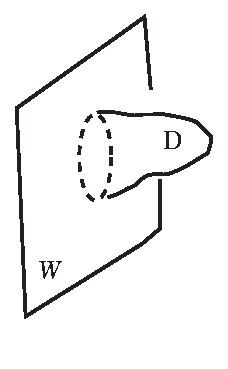
\includegraphics[width=0.28\textwidth,height=0.22\textheight,keepaspectratio]{fig05.pdf}
\caption{一张盘状弦世界面的边界终结在一张 D-膜的世界体 ${\mathcal W}$ 上。}
\end{figure}


首先，条件 \((A')\) 是一个反常抵消的条件。考虑一张弦世界面 \(D\)，其边界落在一张包裹 \({\mathcal W}\times \mathbb{R}\) 的 D-膜上，如图 5 所示。其 \(g\)-函数（示意性地）为 \[g=\int [Dx] [D\psi] ~  e^{-\int_D \partial x \bar \partial x + \psi \partial \psi + \cdots }~~ e^{i \int_D B} ~~ {\mathrm Pfaff}( D/_D) ~ {\mathrm{Tr}}_E Pe^{i \oint_{\partial D} A}\] 路径积分的测度必须在所有如下映射构成的空间上有良好定义： \[\{ x: D \to X_9 \quad: \quad x(\partial D) \subset {{\mathcal W}} \}\] 通过考虑一族路径构成的环路，使得 \(\partial D\) 在 \({\mathcal W}\) 中扫出一块曲面，容易看出：在 de Rham 复形的层面上， \[\iota^*(H_{DR}) = d{\mathcal F}\] 必须能够被平凡化。启发式地，\({\mathcal F}:=F + \iota^*(B)\)，尽管 \(F\) 与 \(\iota^*(B)\) 各自都不是良好定义的。注意，出现在 \(g\)-函数上式中的正是组合 \({\mathcal F}\)，因此它\emph{必须}在膜世界体 \({\mathcal W}\times \mathbb{R}\) 上整体良好定义。方程 \(d{\mathcal F} = \iota^*(H_{DR})\) 意味着 \(H_{DR}\) 是 \({\mathcal F}\) 在膜世界体 \({\mathcal W}\times \mathbb{R}\) 上的一个磁源。

Freed 与 Witten（Freed 等）对整体反常抵消所作的更为细致的分析表明，在整系数上同调的层面上 \[\iota^*[H] + W_3(T{\mathcal W}) =0\] 成立。（另见（Kapustin 等）的讨论。）

\begin{figure}[tbp]
\centering
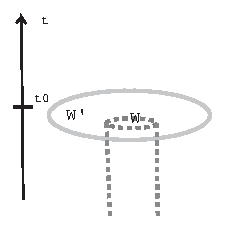
\includegraphics[width=0.28\textwidth,height=0.22\textheight,keepaspectratio]{fig06.pdf}
\caption{包裹空间闭链 ${\mathcal W}$ 的 D-膜在时间中传播，并终结于一个在时间上局域化的位形 ${\mathcal W}'$。这一 D-膜位形是无反常的。}
\end{figure}


现在让我们转向稳定性条件 \((B')\)。假设存在闭链 \({\mathcal W}'\subset X_9\)，使得 \[W_3({\mathcal W}') + [H]\vert_{{\mathcal W}'} \not=0.\] 正如我们刚刚看到的，反常抵消意味着我们不能把 D-膜包裹在 \({\mathcal W}'\) 上。然而，虽然包裹 \({\mathcal W}'\) 的自由膜是有反常的，我们却可以通过为 \({\mathcal F}\) 添加一个磁源来抵消这一反常。一张终结在余维 3 的闭链 \({\mathcal W} \subset {\mathcal W}'\) 上的 D-膜恰好提供这样的磁源。因此，我们可以通过添加一张包裹闭链 \(\mathbb{R}^-\times {\mathcal W}\) 的 D-膜来构造无反常的位形，该膜\emph{终结}于 \({\mathcal W}\subset {\mathcal W}'\)，其中 \({\mathcal W}\) 满足 \[PD({\mathcal W} \subset {\mathcal W}') = W_3({\mathcal W}') + [H]\vert_{{\mathcal W}'}.\] 这里 \(\mathbb{R}^-\) 应被视为时间方向上的半无限区间，如图 6 所示。

图 6 提示了一个清晰的物理解释：一张膜包裹空间闭链 \({\mathcal W}\)，在时间中传播，并终结于一张包裹 \({\mathcal W}'\) 的 D-\emph{``瞬子''}上。这意味着包裹空间闭链 \({\mathcal W}\) 的膜可以是不稳定的，并且会由于包裹 \({\mathcal W}'\) 的位形而衰变。（注：我们为简便起见使用``瞬子''一词，但图 6 所描绘的过程在弦理论中未必是非微扰的。事实上，下文 5.5 节中的例子是\emph{经典}弦理论中的一个过程。该衰变过程只是在时间方向上局域化而已。）其基本机制与 Witten 在 AdS/CFT 对应中讨论过的``重子顶点''密切相关（Witten 等）。

\subsection{经由 Atiyah-Hirzebruch 谱序列与 K-理论的关系}\label{ux7ecfux7531-atiyah-hirzebruch-ux8c31ux5e8fux5217ux4e0e-k-ux7406ux8bbaux7684ux5173ux7cfb}

\((A')\) 与 \((B')\) 事实上正是 K-理论的条件。为了理解这一点，让我们回顾 Atiyah-Hirzebruch 谱序列（AHSS）。设 \(X\) 是一个流形。一个 K-理论类 \(x\in K^0(X)\) 决定了一组整系数上同调类：\(c_i(x)\in H^{2i}(X,\mathbb{Z})\)；而 \(x\in K^1(X)\) 决定了 \(\omega_{2i+1}(x)\in H^{2i+1}(X,\mathbb{Z})\)。现在让我们反过来问：给定一组上同调类 \((\omega_1, \omega_3, \dots)\)，是否存在一个 \(x\in K^1(X)\)？AHSS 是一个逐次逼近的方案：\(E_1^*, E_3^*, E_5^*,\dots\)，用来描述何时这样一组上同调类 \((\omega_1, \omega_3, \dots)\) 来自一个 K-理论类。

为了把 AHSS 与 D-膜联系起来，我们把 \(X\) 中的 \(PD(\omega_k)\) 看作一张空间维数为 \(\dim X - k\) 的（可能不稳定的）膜的空间闭链。这样，一组 \((\omega_1, \omega_3, \dots)\) 就决定了一族膜，因此 AHSS 帮助我们判断 \(X\) 的哪些子簇可以被包裹。现在让我们更仔细地考察 AHSS：

第一个近似就是 D-膜的上同调分类： \[\begin{matrix}
K^0(X) \sim   E^0_1(X) & :=   H^{\mathrm even}(X,\mathbb{Z}) \\
K^1(X) \sim  E^1_1(X) & :=  H^{ \mathrm odd}(X,\mathbb{Z})
\end{matrix}\] 第一个非平凡的近似是 \[\begin{matrix}
K^0(X) \sim E^0_3(X) &  := \bigl( {\mathrm Ker} ~d_3\vert_{H^{\mathrm even} }\bigr) / \bigl({\mathrm Im} ~d_3\vert_{H^{\mathrm odd}}\bigr)\\
K^1(X) \sim E^1_3(X)  & := \bigl( {\mathrm Ker} ~d_3\vert_{H^{\mathrm odd} }\bigr) / \bigl({\mathrm Im} ~d_3\vert_{H^{\mathrm even}}\bigr)
\end{matrix}\] 其中 \[d_3(a) := Sq^3(a) + [H]\smile a.\]

我们停下来定义一下 \(Sq^3(a)\)。为简单起见，假设 Poincaré 对偶 \(PD(a)\) 可以由一个流形 \({\mathcal W}\) 代表，并令 \(\iota: {\mathcal W} \hookrightarrow X_9\) 为包含映射。于是我们令 \[Sq^3(a) = \iota_*(W_3({\mathcal W}) )\] 其中 \(\iota_*\) 是三个操作的复合：先取 \(W_3({\mathcal W})\) 在 \({\mathcal W}\) 内的 Poincaré 对偶，然后把该同调闭链前推，最后在 \(X_9\) 中取 Poincaré 对偶。等价地，把 \(a\) 视为紧支撑在 \({\mathcal W}\) 的管状邻域中的类，并考虑类 \(W_3({\mathcal W}) \smile a\)，其中 \(W_3({\mathcal W})\) 被拉回到该管状邻域。

回到 AHSS。一般来说，必须继续这一逼近方案。例如，在计算 \(N\geq 3\) 的 \(SU(N)\) 的扭曲 K-理论时便是如此。

现在，让我们用物理语言来解释取 \(d_3\) 上同调这一程序。为了解释 \({\mathrm Ker }~ d_3\)，注意由上式可得 \[d_3(a)=0 \quad \Leftrightarrow \quad
\biggl( W_3({\mathcal W}) + [H] \biggr) \smile a = 0 .\] 回忆一下，包裹 \({\mathcal W}\) 的 D-膜的整体反常抵消意味着 \[W_3({\mathcal W}) + [H]\vert_{{\mathcal W}} =0\] 而这又蕴涵 \(d_3(a)=0\)。因此，物理条件 \((A')\) 蕴涵 \(PD({\mathcal W}) \in {\mathrm Ker} d_3\)。

其次，让我们解释上式中对 \(d_3\) 的像取商这一步骤。假设 \(a=d_3(a') = (Sq^3 + [H])(a')\)。于是选取代表 \[PD(a) = {\mathcal W} \qquad  PD(a') = {\mathcal W}' ,\] 其中 \({\mathcal W}\) 在 \({\mathcal W}'\) 中余维为 3。一张终结于 \({\mathcal W}\) 上的 \(D\)-膜可以作为 \({\mathcal W}'\) 上 D-膜规范场的磁源，并且 \[PD\bigl( {\mathcal W} \hookrightarrow {\mathcal W}' \bigr)
= W_3({\mathcal W}') + [H]\vert_{{\mathcal W}'} ~~ \Rightarrow ~~a = d_3(a')\] 因此，D-瞬子导致膜不稳定的这一物理过程意味着，我们应当对 \(d_3\) 的像取商（Diaconescu 等；Maldacena 等）。（事实上，条件 \((A'),(B')\) 所包含的信息比 \(d_3\) 更多。）

\subsection{\texorpdfstring{例子：\(SU(N)\) 的扭曲 K-群}{例子：SU(N) 的扭曲 K-群}}\label{ux4f8bux5b50sun-ux7684ux626dux66f2-k-ux7fa4}

作为上述观点的一个说明，让我们考察 \(SU(2)\) 与 \(SU(3)\) 的扭曲 K-群。

先考虑 \(K_H(SU(2))\)。此时 \(H=k \omega\)，其中 \(\omega\) 生成 \(H^3(SU(2);\mathbb{Z})\)。在膜的上同调模型中我们有 \(H^{\mathrm even}(SU(2))= H^0 \cong H_3= \mathbb{Z}\)，对应于``D3-膜''（或 D2-瞬子）；而 \(H^{\mathrm odd}(SU(2))= H^3 \cong H_0 = \mathbb{Z}\)，对应于``D0-膜''。现在条件 \((A')\) 表明我们只能有 D0-膜。确实，包裹 \(SU(2)= S^3\) 的 D2-瞬子会以 \(k\) 个单位为量破坏 D0-膜荷，如图 7 所示。由于这个原因，若我们取 \(SU(2)\) 作为条件 \((B')\) 中的闭链 \({\mathcal W}'\)，则可推出：含 \(k\) 张 D0-膜的体系与完全不含 D0-膜的体系处于 \({\mathcal B}\) 的同一连通分支之中。在 5.5 节中我们将更详细地解释这如何可能。

\begin{figure}[tbp]
\centering
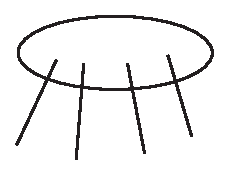
\includegraphics[width=0.28\textwidth,height=0.22\textheight,keepaspectratio]{fig07.pdf}
\caption{在 $SU(2)$ 第 $k$ 层理论中，$k$ 张 D0-膜终结于一张包裹的 D2-膜瞬子上。}
\end{figure}


由此我们得出结论： \[\begin{matrix}
K^0_H(SU(2)) & = 0 \\
K^1_H(SU(2)) & = \mathbb{Z}/k\mathbb{Z}
\end{matrix}\] 这确实也容易由严格的数学论证加以确认。

现在让我们考虑 \(K_H(SU(3))\)。这里 AHSS 不足以确定该 K-群。然而，重要的是要记住：物理条件 \(A',B'\) 所含的信息比 \(d_3\)-上同调更多，也更强。我们仍然取 \(H=k \omega\)，其中 \(\omega\) 生成 \(H^3(SU(3);\mathbb{Z})\)。

在上同调模型中我们有 \(H^{\mathrm odd} \cong H_3 \oplus H_5\)。现在，3-膜不能包裹 \(SU(2)\subset SU(3)\)，因为 \([H]_{DR}\not=0\)。但 5-膜可以包裹闭链 \(M_5\subset SU(3)\)，其中 \(M_5\) 是 \(\omega\) 的 Poincaré 对偶。现在， \[\int_{SU(3)} \omega Sq^2 \omega = 1\] 因此 \[\iota^*(\omega) = W_3(M_5)\] 非零。（事实上，闭链 \(M_5\) 可以由对称 \(SU(3)\) 矩阵构成的空间来代表。该空间微分同胚于 \(SU(3)/SO(3)\)，是非 Spin\(^c\) 流形的一个简单例子。）

由上式可知，若 \(M_5\) 被包裹 \(r\) 次，反常抵消意味着 \[r(k+1) W_3 = 0\] 与条件 \((B')\) 相关的 D-膜瞬子正是包裹 \(SU(2)\) 的那些 \(D2\)-膜。于是我们得出结论： \[K^1_{H=k\omega}(SU(3))  = \begin{cases}
 \mathbb{Z}/k\mathbb{Z} & k\ \text{为奇数}  \\
  2\mathbb{Z}/k\mathbb{Z} & k\ \text{为偶数}
 \end{cases}\]

现在让我们转向偶数维的膜，\(H^{\mathrm even} \cong H_0 \oplus H_8\)。8-膜是有反常的，因为 \([H]_{DR}\not=0\)；但 \(0\)-膜是无反常的。

\begin{figure}[tbp]
\centering
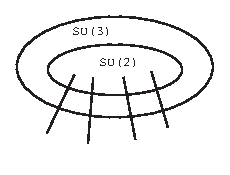
\includegraphics[width=0.28\textwidth,height=0.22\textheight,keepaspectratio]{fig08.pdf}
\caption{$k$ 张 D0-膜终结于 $SU(3)$ 的某个 $SU(2)$ 子群中一张包裹的 D2-膜瞬子上。}
\end{figure}


\begin{figure}[tbp]
\centering
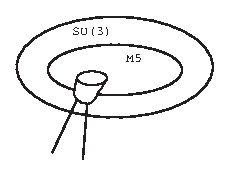
\includegraphics[width=0.28\textwidth,height=0.22\textheight,keepaspectratio]{fig09.pdf}
\caption{当 $k$ 为偶数时，$\frac{1}{2} k$ 张 D0-膜可以终结于 $SU(2)$ 的一个半球面上，而该半球面终结于 $H_5(SU(3),\mathbb{Z})$ 的一个生成元上。}
\end{figure}


现在，由于图 8 的标准过程，D0-膜荷并不守恒。然而还存在一个更微妙的瞬子，如图 9 所示：其中一条 3-链终结于 \(H_2(M_5;\mathbb{Z})\cong \mathbb{Z}_2\) 中的一个非平凡元素上。当 \(k\) 为偶数时，这个瞬子以 \(\frac{1}{2} k\) 个单位为量破坏 D0 荷。由此我们得出结论： \[K^0_{H}(SU(3)) = \begin{cases}
   \mathbb{Z}/k\mathbb{Z} & k\ \text{为奇数} \\
   \mathbb{Z}/\frac{k}{2}\mathbb{Z}  & k\ \text{为偶数}
   \end{cases}\]

人们大概可以把上述程序推广（至少对 \(SU(N)\)）用到 Steenrod 的胞腔分解，来计算更高秩群的扭曲 K-理论，但这一点尚未被做出来。部分地受上述结果（以及下一节将解释的 D0 荷量子化结果）的启发，M. Hopkins 严格地计算了 \(SU(N)\) 的扭曲 \(K\)-同调。他发现，对于 \(H=k\omega\)： \[K_{H,*}(SU(N)) =
(Z/d_{k,N} Z)\otimes \Lambda_Z[w_5, \dots, w_{2N-1}]\] 其中 \[d_{k,N}  = {\mathrm gcd}\bigl[\binom{k}{1}, \binom{k}{2},
\dots, \binom{k}{N-1}\bigr].\] 我们发现在上面对 \(G=SU(2),SU(3)\) 的情形完全吻合。

把上式与 \[H_*(SU(N)) = \Lambda_Z[w_3, w_5, \dots, w_{2N-1}].\] 相比较是很有意思的。回忆一下，在有理同调的意义下 \(SU(N) \sim S^3 \times S^5 \times \cdots S^{2N-1}\)。显然，拓扑上不同的 D-膜可以被描绘为包裹 \(SU(N)\) 中不同的闭链，但要受某些衰变过程的约束。在下一节中我们将回到世界面重整化群的观点，来解释这些衰变过程中最重要的一个。我们还将给出一个简单的物理论证（它实际上早于 Hopkins 的计算），说明为什么荷群应当是阶为 \(d_{k,N}\) 的挠群。

\SrcRange{23}{36}
\section{\texorpdfstring{\(SU(N)\) WZW 模型中膜的例子}{SU(N) WZW 模型中膜的例子}}\label{sun-wzw-ux6a21ux578bux4e2dux819cux7684ux4f8bux5b50}

在本节中，我们将运用``保持对称性的膜''（symmetry-preserving branes）的理论，来确定 \(SU(N)\) 第 \(k\) 级 WZW 模型中 D0 荷群的阶 \(d_{k,N}\)。这一论证的不同版本见 文献。关于本节材料的进一步细节的综述，见 文献 及其中的参考文献。

让我们在此概述该论证的策略：

\begin{itemize}
\item
  我们借助边界共形场论的形式，以代数方式定义``基本的''或``单次缠绕的''保持对称性的边界条件。这些边界条件由中心扩张环路群的幺正不可约表示 \(\lambda \in P^+_k\) 标记。
\item
  我们给出这些边界条件的半经典图像：它们作为膜缠绕在带有非平凡 Chan-Paton 线丛的特殊正则共轭类上。见下文方程 (5.14) 与 (5.24)。
\item
  接着我们讨论何以``多次缠绕的''保持对称性的膜能够位于 \({\mathcal B}\) 中对应于某些单次缠绕膜的连通分支之内。例如，``由 \(L\) 张 D0 膜构成的堆叠''可以通过重整化群流连续地连接到由 \(\lambda\) 标记的保持对称性的膜，只要 D0 膜的数目 \(L\) 等于群 \(G\) 的表示 \(\lambda\) 的维数 \(d(\lambda)\)。
\item
  这意味着保持对称性的膜 \(\lambda\) 在某种意义上带有 D0 荷 \(L\)。另一方面，正如我们在上一节所见，D0 荷必须是有限阶的并且是循环的。因此 D0 荷为 \(d(\lambda) {\mathrm mod} d_{k,N}\)，其中 \(d_{k,N}\) 为某个整数。
\item
  最后我们指出，对应于不同 \(\lambda\) 值的保持对称性的膜有时可以通过与恒等变换连续相连的刚性旋转相联系。这样的膜显然处于 \({\mathcal B}\) 的同一连通分支中，而这就足以确定挠群的阶 \(d_{k,N}\)。
\end{itemize}

\subsection{\texorpdfstring{\(G=SU(N)\) 的 WZW 模型}{G=SU(N) 的 WZW 模型}}\label{gsun-ux7684-wzw-ux6a21ux578b}

让我们先约定记号。WZW 场 \(g: \Sigma \to G\) 的作用量为 \[S = \frac{k}{8 \pi} \int_{\Sigma}   {\mathrm{Tr}}_N [
(g^{-1}\partial g) (g^{-1}\bar{\partial}  g)] + {2 \pi k } \int \omega\] 其中迹取在基本表示中。靶空间 \(G=SU(N)\) 具有度规 \[ds^2 = -\frac{k}{2} {\mathrm{Tr}}_N (g^{-1}dg\otimes g^{-1} dg)\] 以及场强为下式的``\(B\)-场'' \[H = k \omega, \qquad   \quad \omega:= -\frac{1}{24 \pi^2}{\mathrm{Tr}}(g^{-1} dg)^3\] 其中 \([\omega]\) 生成 \(H^3(G;Z) \cong Z\)。CFT 态空间为 \[{\mathcal H}^{\mathrm closed} \cong \oplus_{\mathrm P^+_k} {\mathcal H}_\lambda \otimes \tilde {\mathcal H}_{\lambda^*}\] 其中 \({\mathcal H}_{\lambda},  \tilde {\mathcal H}_{\lambda^*}\) 是环路群 \(\widetilde{LG}_k\) 的左行与右行幺正不可约表示，如 文献 所述。

在共形边界条件（即膜）的集合之中，有一组特殊的``保持对称性的边界条件''，它们使左右行流之和 \(J + \tilde J\) 的对角和保持不被破坏。更多细节见 文献。由于存在未破缺的仿射对称性，开弦态射空间 \({\mathcal H}_{ab}^{\mathrm open}\) 本身也是 \(\widetilde{LG}_k\) 的表示。相应地，它们是按 \(\lambda\in P^+_k\) 标记的边界条件范畴中的对象。态射空间按 \(\widetilde{LG}_k\) 的不可约表示所作出的分解由下式给出 \[{\mathcal H}_{\lambda_1, \lambda_2}^{\mathrm open}
 = \oplus_{ \lambda_3\in P^+_k} N^{  \lambda_3}_{\lambda_1, \lambda_2} {\mathcal H}_{  \lambda_3}\] 其中 \(N^{  \lambda_3}_{\lambda_1,
\lambda_2}\) 为融合系数。

建立上式最有效的方式是通过``边界态形式''。在第 2 节的二维拓扑场论中，与边界条件 \(a\) 相伴的边界态定义为 \(\iota^{a}(1_a)\)，其中 \(1_a\) 是开弦代数 \({\mathcal H}_{aa}\) 中的单位元。它是闭弦代数 \({\mathcal C}\) 中的一个元素，该元素``生成''一个具有边界条件 \(a\) 的自由边界。类似地，在边界 CFT 中，对每一个共形边界条件 \(a\) 都相伴一个相应的``边界态'' \[\vert B(a)\rangle\rangle \in {\mathcal H}^{\mathrm closed}.\] 对于保持对称性的 WZW 边界条件，相应的边界态由 Cardy 公式给出： \[\vert B(\lambda) \rangle\rangle= \sum_{\lambda'\in P^+_k} {S_{\lambda}^{~\lambda'} \over \sqrt{
S_{0}^{\lambda'} }} ~ {\mathbf 1}_{{\mathcal H}_{\lambda'}} \in {\mathcal H}^{\mathrm closed}\] 其中 \(S_{\lambda}^{~\lambda'}\) 为模 \(S\)-矩阵，\(0\) 表示基本表示，并且我们把闭弦态空间理解为： \[{\mathcal H}^{\mathrm closed}
\cong \oplus_{ P^+_k} {\mathcal H}_\lambda \otimes \tilde {\mathcal H}_{\lambda^*}
  \cong
 \oplus_{ P^+_k}   {\mathrm Hom}({\mathcal H}_{ \lambda} , {\mathcal H}_{\lambda} )\] 对上式应用 Cardy 条件即得所需表达式。

由于圆盘配分函数是基态与边界态的重叠，\(Z_{\mathrm disk} = \langle 0 \vert B(\lambda)\rangle\rangle\)，这些共形不动点的 \(g\)-函数可立即由上式得到： \[g(\lambda) = S_{\lambda,0}/\sqrt{S_{00}} .\]

最后，正如我们先前所指出的，为了让膜能够稳定存在，引入世界面超对称是至关重要的。引入 \({\mathcal N}=1\) 超对称即已足够，尽管当嵌入到 II 型弦背景中时，整个背景可以具有 \({\mathcal N}=2\) 超对称。同样重要的是，共形场论上要有定义良好的 \((-1)^F\) 作用。这区分了 \(G\) 的秩为奇数和偶数的情形。当秩为奇数时，我们总可以添加一个 \({\mathcal N}=1\) 的 Feigin-Fuks 超场，这在构建 II 型弦背景时确实十分自然。

\subsection{保持对称性的膜的几何解释}\label{ux4fddux6301ux5bf9ux79f0ux6027ux7684ux819cux7684ux51e0ux4f55ux89e3ux91ca}

我们想讨论由 \(\lambda\) 标记的保持对称性的边界条件的\emph{几何}解释。也就是说，我们希望得到把膜视为群流形中延展对象的某种半经典图像。本节说明这一图像是如何导出的。

让我们先回顾 WZW 模型中紧致靶空间的几何是如何恢复的。在 WZW 模型中度规正比于 \(k\)，故路径积分测度带有权重因子 \[\sim e^{ - k S}\] 因此，我们预期半经典图像会在 \(k\to \infty\) 极限下浮现。在此极限下，顶点算子代数``退化''成为群 \(G\) 上的函数代数。例如，CFT 关联函数变成群流形上的积分： \[\langle \hat F_1(g(z_1,\bar z_1)) \cdots  \hat F_n(g(z_n,\bar z_n))\rangle
\to \int_G d\mu(g) F_1(g)\cdots F_n(g)\] 在左侧，\(\hat F_i\) 是维数 \(\sim 1/k\) 的适当顶点算子。在右侧，\(F_i\) 是 \(G\) 上相应的 \(L^2\) 函数。粗略地说，CFT 态空间退化为 \[{\mathcal H}^{\mathrm closed}
\cong \oplus_{\mathrm P^+_k} {\mathcal H}_\lambda \otimes \tilde {\mathcal H}_{\lambda^*}
\rightarrow L^2(G)\otimes {\mathcal H}^{\mathrm string}\] 其中 \(L^2(G)\) 是初级场的极限，\({\mathcal H}^{\mathrm string}\) 包含``振子激发''。在此极限下边界态退化： \[\vert B(\lambda)\rangle\rangle
\to B_\lambda  + \cdots\] 其中 \(B_\lambda\in L^2(G)\)，并在 \(k \to \infty\) 极限下成为一个分布。虽然前者显然只是启发式的，后者却有明确的含义，因为 \(\vert B(\lambda) \rangle\rangle\) 与维数 \(\sim 1/k\) 的初级场的重叠具有定义良好的极限。

\begin{figure}[tbp]
\centering
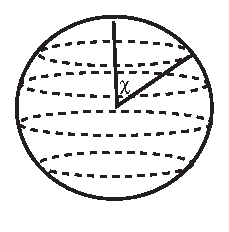
\includegraphics[width=0.28\textwidth,height=0.22\textheight,keepaspectratio]{fig10.pdf}
\caption{$SU(2)$ 中的特殊共轭类。这些是保持对称性的膜的半经典世界体积。}
\end{figure}


利用方程上述方程、模 \(S\)-矩阵的公式以及 Peter-Weyl 定理，可以求得函数 \(B_\lambda\) 集中在正则共轭类 \[{\mathcal O}_{\lambda,k}:= \biggl[ \exp\bigl(2\pi i \frac{\lambda + \rho}{k + h}  \bigr)\biggr]\] 之上，从而得到上图所示的膜的半经典图像。这里 \(\rho\) 是 Weyl 向量，\(h\) 是对偶 Coxeter 数。（照例，在超对称情形应作替换 \(k \to k-h, \lambda\in P^+_{k-h}\)。）更多细节见 文献。

评注：

\begin{itemize}
\item
  由于 \(k\) 是半经典展开参数，我们只能期望在用闭弦顶点算子时把膜定位到长度尺度 \(\ell_{\mathrm string} \sim 1/\sqrt{k}\) 的精度之内 文献。设 \(\underline{\mathbf{t}}\) 为极大环面的 Lie 代数，并令 \(\mathrm{ch}i\in \underline{\mathbf{t}}\) 参数化共轭类。则度规 \(ds^2 \sim k (d\mathrm{ch}i)^2\)，因此顶点算子只能``分辨''角度 \(\delta \mathrm{ch}i\geq {1\over \sqrt{k}}\)。这一不确定度涵盖了上述公式中许多不同的共轭类。然而，半经典几何图像对许多重要的物理量给出精确结果。其原因在于，相关的精确 CFT 结果是 \(1/k\) 的多项式，因而可以在半经典展开中精确计算。
\item
  基本表示 \(\lambda=0\) 给出``最小的''膜。我们将称之为``D0-膜''。在用 WZW 模型构建的 IIA 型弦紧致化中，该态被用来构造 D0 膜。但要注意，在此描述中它\emph{并非}点状的，而是具有量级为弦长 \(\sim 1/\sqrt{k}\) 的大小。
\end{itemize}

\subsection{用 CFT 测量膜之间的距离}\label{ux7528-cft-ux6d4bux91cfux819cux4e4bux95f4ux7684ux8dddux79bb}

为了进一步支持上面所主张的几何图像，让我们说明 D-膜可以在群中转动，并且膜之间的距离随后可以用 CFT 技术来测量。

首先，我们说明如何``转动''D-膜。\(G_L \times G_R\) 作用在 \({\mathcal H}^{\mathrm closed}\) 上，因此我们可以考虑边界态 \[g_L  g_R\vert B(\lambda) \rangle\rangle.\] 在 \(k\to \infty\) 极限下，该态具有类似于上述公式的极限。特别地，它支撑在子集 \[g_L {\mathcal O}_{ \lambda,k } g_R \subset G.\] 之上。

\begin{figure}[tbp]
\centering
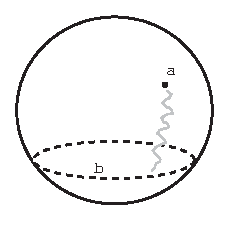
\includegraphics[width=0.28\textwidth,height=0.22\textheight,keepaspectratio]{fig11.pdf}
\caption{用 D0 膜作为边界条件 $a$，我们可以通过研究拉伸弦的最低质量来探测膜 $b$ 的位置。}
\end{figure}


现在，让我们考虑开弦态空间 \({\mathcal H}_{ba}^{\mathrm open}\)，其中 \(a\) 对应于转动后的 D0 膜，\(a= g_L\cdot \vert B(\lambda=0)\rangle\rangle\)，而 \(b=\vert B(\lambda)\rangle\rangle\)。该空间中的典型弦可如图 11所描绘。这一图像提示了``测量''两膜之间距离的方法，从而可以按照 文献 的精神来定义膜的位置。该图像表明，开弦通道配分函数在小 \(q_o\) 下有展开 \[{\mathrm{Tr}}_{{\mathcal H}_{b,a}^{\mathrm open} } q_o^{L_0}
~~ \stackrel{?}{= } ~~
q_o^{(T_f D)^2 } + \cdots\] 其中 \(D\) 是位于 \(g_L\) 处的 \(D0\) 膜中心与膜 \(b\) 之间的测地距离。\(T_f\) 是基本弦张力（此处我们取 \(\alpha'=1\)，故 \(T_f = 1/(2\pi)\)）。

我们实际上可以用边界态的表达式以及 Cardy 条件来计算上述表达式的 \(q_o\) 展开： \[{\mathrm{Tr}}_{{\mathcal H}_{b,a} } q_o^{L_0 - c/24 } =
\langle\langle B(\lambda)\vert q_c^{\frac{1}{2} ( L_0 + \tilde L_0 - c/12)} \rho_L(g ) \vert B(0)\rangle\rangle\] 其中 \(q_c = e^{2\pi i \tau_c}\)，\(q_o = e^{-2\pi i /\tau_c}= e^{2\pi i \tau_o}\)。计算是直接的。让我们给出 \(SU(2)\) 的结果。若 \(g_L\) 共轭于 \[\begin{pmatrix} e^{i \mathrm{ch}i}& 0 \\ 0 & e^{- i \mathrm{ch}i}\\\end{pmatrix}\] 且 \(0 \leq \mathrm{ch}i \leq \pi\)，则在 Ramond 扇区中，上式里 \(q_o\) 的最低次幂为 \[k \left( \frac{\hat{\mathrm{ch}}i_j - \mathrm{ch}i}{2\pi } \right)^2 .\] 这里 \(\hat{\mathrm{ch}}i_j = \pi (2j+1)/k\)，而膜 \(b\) 由 \(j\in \{0, \frac{1}{2}, \dots, \frac{k-2}{2} \}\) 标记。公式上述公式\emph{恰好}就是 \((T_f D)^2\)，正如朴素预期的那样。我们再次看到，膜的几何图像被共形场论优美地再现出来。\TN{在玻色情形，上述公式实际上是 \(\frac{k+2}{4} \left( \frac{\hat{\mathrm{ch}}i_j - \mathrm{ch}i}{\pi } \right)^2 +\frac{1}{2} \frac{\mathrm{ch}i}{\pi}(1-\frac{\mathrm{ch}i}{\pi} )- \frac{1}{4( k+2)}\)，所以只有当 \(k(\delta \mathrm{ch}i)^2 \gg 1\) 时结论才成立。}对于陪集模型中的 D-膜也有非常类似的评述 文献。

\subsection{膜为什么稳定？}\label{ux819cux4e3aux4ec0ux4e48ux7a33ux5b9a}

前几节所主张的几何图像引出一个有趣的疑难。我们现在来描述这个疑难，以及它在 文献 中的优美解决。

考虑一张膜如图 10那样一次缠绕 \({\mathcal O}_{\lambda,k}\subset G\)。在 II 型弦理论的语境中，膜具有非零张力 \(T\)，其单位为能量/体积。因此，用膜缠绕一个子流形 \({\mathcal W}\) 要消耗能量 \(E\sim T{\mathrm vol}({\mathcal W})\)。然而，正则共轭类 \({\mathcal O}_{\lambda,k} \subset G\) 在同调上是平凡的。例如，对 \(SU(2)\)，\({\mathcal O}=S^2\subset S^3\)。因此我们预期该膜不稳定，会收缩为一点。

这导致一个悖论：我们从共形场论知道该膜是绝对稳定的。由边界态的表达式，我们可以从 \[{\mathrm{Tr}}_{
{\mathcal H}_{\lambda, \lambda} } q^{L_0 - c/24}\] 计算开弦态空间中算子的谱，并发现所有 \(\Delta_i\geq 1\)。根据上式可知，不存在离开该点的 \(\beta\) 下的不稳定流！

悖论的解决在于这样一个事实：D-膜上也有规范场自由度。膜携带一个带联络的 \(U(1)\) 线丛 \({\mathcal L} \to {\mathcal O}\)。若该丛是扭曲的，则存在一种与张力相抗衡的稳定化力。

为以最简单的方式说明这一解决，考虑 \(SU(2)\) 中半径为 \(R=\sqrt{k}\sin \mathrm{ch}i\) 的共轭类 \({\mathcal O} = S^2\) 的例子。若膜的 Chan-Paton 线丛的 Chern 类为 \(n\in \mathbb{Z}\)，则 \(\int_{{\mathcal O}} F = 2\pi n\)。由此可知 Yang-Mills 作用量为 \[\int_{S^2} F\wedge * F \sim \frac{n^2}{R^2}\] 因此我们可以计算 \(g\)-函数见上式 \[g(\mathrm{ch}i) \sim R^2 + \frac{n^2}{R^2 }\] 它在 \(\mathrm{ch}i \sim \pi n/k\) 处取极小，因此我们预期 \({\mathcal B}\) 中由 \(n\) 决定的扇区中的重整化群流会演化到这一位形。

上述论证已由 \(SU(2)\) 推广到高秩群 文献。所得到的结论是，\(\vert B(\lambda) \rangle\rangle\) 可以半经典地图像为缠绕共轭类 \({\mathcal O}_{  \lambda,k}\)。膜为单次缠绕，其 Chan-Paton 线丛 \({\mathcal L}_{  \lambda} \to {\mathcal O}_{  \lambda,k}\) 具有第一 Chern 类 \[c_1({\mathcal L}_{  \lambda}) =   \lambda + \rho \in H^2(G/T;Z) \cong \Lambda_{\mathrm weight}.\] （进一步的细节见 文献。）

研究此问题中的 \(g\)-函数及其 DBI 作用量近似是很有意思的。我们把注意力限制在玻色 WZW 模型。设 \(\mathrm{ch}i\) 参数化 \(G\) 中的共轭类。对于上述 Chan-Paton 线丛中的 Chan-Paton 线丛，作为 \(\mathrm{ch}i\) 的函数的 DBI 作用量 \[g_{DBI}(  \mathrm{ch}i) := \int_{{\mathcal O}_\mathrm{ch}i} \sqrt{\det(g+ F+B)}\] 在 \(\mathrm{ch}i_* = 2\pi (\lambda + \rho)/(k+h)\) 处取极小，其值为： \[g_{DBI}(\mathrm{ch}i_*)/g_{DBI}(0) = \prod_{\alpha>0 } \biggl({k \sin \frac{1}{2} \alpha \cdot \mathrm{ch}i\over \pi
\alpha\cdot \rho}\biggr).\] 这里乘积遍历正根。这与精确的 CFT 结果 \[g(\lambda)/g(0) =
\prod_{\alpha>0 } \biggl(\frac{\sin \pi \alpha \cdot (\lambda+\rho)/(k+h)}{\sin \pi \alpha \cdot  \rho/(k+h)  }\biggr).\] 吻合得出奇地好。注意右边正是量子维数 \(d_q(\lambda)\)，与上面的上面的公式和谐一致。

\subsection{D0 膜的集合如何演化为保持对称性的膜}\label{d0-ux819cux7684ux96c6ux5408ux5982ux4f55ux6f14ux5316ux4e3aux4fddux6301ux5bf9ux79f0ux6027ux7684ux819c}

我们刚才描述的保持对称性的膜的半经典图像引出一个重要的新论点。在 II 型弦紧致化中，若膜携带拓扑非平凡的 Chan-Paton 丛，则它携带非平凡的诱导 D-膜荷。在目前情形，由于 Chan-Paton 线丛满足 \(\int_{{\mathcal W}} e^{c_1({\mathcal L})}\not=0\)，故它携带 D0 荷。这提示：由 \(\vert B(\lambda) \rangle\rangle\) 刻画的共形不动点与对应于``一组 D0 膜''的不动点处于 \({\mathcal B}\) 的同一连通分支之中。本节回顾为何这是对的。\TN{实际上，用 Feigin-Fuks 超场把 \(SU(2)\) WZW 模型最显然地嵌入 IIA 型背景，所得出的背景其 RR D0 荷的定义其实是微妙的。相关的 \(U(1)\) RR 规范群由于荷为 \(k\) 的时空标量场凝聚而自发破缺为 \(\mathbb{Z}_k\)。更多讨论见 文献。}

物理学家所说的``D0 膜堆叠''是指对某个正整数 \(L\) 的边界态 \(L \vert B(0)\rangle\rangle\)。按定义，这样的 D0 膜堆叠的开弦扇区具有态空间 \[{\mathcal H}_{L B(0) , b }^{\mathrm open} = \mathbb{C}^L \otimes {\mathcal H}_{B(0),b}^{\mathrm open}\] 对任意边界条件 \(b\) 成立。

\emph{断言}：若 \(\lambda\in P_k^+\) 且 \(L=d(\lambda)\)，则 \(L \vert B(0)\rangle\rangle\) 与 \(\vert B(\lambda)\rangle\rangle\) 处于 \({\mathcal B}\) 的同一连通分支。

注意 \[\frac{g(B(\lambda))}{g(LB(0) )} = {S_{\lambda,0}\over L S_{00}} = \frac{d_q(\lambda)}{d(\lambda)} < 1\] 故该断言与 \(g\)-定理很好地相容。特别地，若这些不动点可由重整化群流连接，则 \(L\) 张 D0 膜不稳定而衰变为 \(\lambda\)，反之则不然。我们有时把这一不稳定性称为``吹胀效应''（blowing up effect）。

所涉及的 RG 流出现在 Kondo 效应的理论中，并由 Affleck 与 Ludwig 研究过 文献。他们的结果被 Schomerus 及其合作者应用于目前的情境。见 文献 及其中的参考文献。Kondo 模型的轨道是通过用某个表示中未破缺流代数的和乐来微扰共形不动点而得到的。应当把 \(L \vert B(0)\rangle\rangle\) 变为 \(\vert B(\lambda)\rangle\rangle\) 的这条流，由考虑圆盘配分函数给出 \[Z(u) = \langle {\mathrm{Tr}}_{\lambda}\biggl( P \exp \oint d\tau u J(\tau) \biggr)\rangle.\] 正如 文献 中所解释的，Affleck 与 Ludwig 的结果支持了主要断言。

实际上，在此问题中考虑 \({\mathcal N}=1\) 超对称是重要的。\TN{下面的论证综合了 文献 中的要素。}在超对称 WZW 模型中我们有一个超场 \[{\mathbf J}_a(z) = \psi_a(z) + \theta I_a(z),\] 其中我们为 Lie 代数选取了正交归一基，以 \(a=1, \dots, \dim G\) 标记。OPE 为 文献 \[\begin{matrix} I_a(z) I_b(w) & \sim {k
\delta_{ab}\over (z-w)^2} +  f_{ab}^{~~c} \frac{I_c(w)}{z-w}
+\cdots \\ I_a(z) \psi_b(w) & \sim {f_{ab}^{~~c}
\psi_c(w)\over z-w} + \\ \psi_a(z) \psi_b(w) & \sim {k
\delta_{ab}\over (z-w)} +\cdots \end{matrix}\] 按标准论证，流 \(J_a = I_a + \frac{1}{2k} f_{abc} \psi_b \psi_c\) 与费米子退耦，并满足能级为 \(k-h\) 的流代数。Hamiltonian 与超对称荷（在 Ramond 扇区中）由下式给出 \[\begin{matrix}
Q & = \oint dz  \biggl( \frac{1}{k} J_a \psi_a - \frac{1}{6k^2} f_{abc} \psi_a \psi_b \psi_c \biggr) \\
H & =\frac{1}{2k} \oint dz  \left( :J_a J_a: +  \partial \psi_a \psi_a \right) \end{matrix}\] 超对称变换为 \([Q,\psi_a] = I_a\) 与 \([Q, I_a] = \partial \psi_a\)。

现在，让我们添加一个保持 \({\mathcal N}=1\) 超对称的类 Kondo 边界微扰。这通过选取 \(G\) 的一个表示 \(\lambda\) 并取下式来给出 \[g(u) = \langle {\mathrm{Tr}}_{\lambda}\biggl( P \exp \oint d\tau u I(\tau) \biggr)\rangle\] 利用 \([Q, I_a] = \partial \psi_a\) 对上述受微扰的作用量中受微扰的作用量作变分，我们可以计算受微扰的超荷 \(Q_u\)。该算子作用在 \(\mathbb{C}^L \otimes {\mathcal H}^{\mathrm open}\) 上为 \[\begin{matrix}
Q_u & = Q+ u \psi^a(0)  S^a\\
&  = Q+ u \sum_{n\in \mathbb{Z}}  \psi^a_n S^a \end{matrix}\] 在第一行中我们转到了 \([0,\pi]\) 上开弦的 Hamiltonian 形式（且我们只修改 \(\sigma=0\) 处的边界条件），并引入了群 \(G\) 的有限维表示 \(\mathbb{C}^L\) 的显式生成元 \(S^a\)。在第二行中我们用了加倍技巧，把结果用平面 \(\mathbb{C}\) 上单值手征顶点算子的模来表示。我们现在可以计算受微扰的 Hamiltonian \[H_u = Q_u^2 = H + u I^a(0)S^a + u^2 (\psi^a(0) S^a)^2\] 上式中第三项是奇异的，但该项的重整化由超对称的要求所固定。Hamiltonian 可以写成 \[\begin{matrix}
& H_u= \frac{1}{2k} \sum_n \left( : (J^a_n + uk S^a)(J^a_{-n} + uk S^a) : + n \psi^a_n \psi^a_{-n} \right)  \\
& + \frac{1}{2} u (u-\frac{1}{k}) \sum_{n,m} f^{abc} \psi_n^a \psi_m^b S^c \end{matrix}\] 因此理论的真空作为 \(u\) 的函数以复杂的方式演化。注意，恰在 \(u=u_*=1/k\) 时，Hamiltonian 简化为 \[H_* = \frac{1}{2k} \sum_n \left( : {\mathcal J}^a_n {\mathcal J}^a_{-n} : + n \psi^a_n \psi^a_{-n} \right)\] 其中 \[{\mathcal J}^a_n  := J^a_n + S^a\] 也满足能级为 \(k-h\) 的流代数。因此，在 \(u=u_*\) 处，我们可以用这些流构造一个新的超共形代数。

上一段强烈提示 \(u_*=1/k\) 是边界共形场论的第二个临界点。现在，我们可以利用 Affleck 与 Ludwig 的一个观察。若 \({\mathcal H}_{\lambda'}\) 是 \(J_n^a\) 的表示，则关于新的流代数 \({\mathcal J}_n^a\) 我们可以作分解： \[\mathbb{C}^L\otimes {\mathcal H}_{\lambda'} \cong \oplus_{\lambda''\in P^+_k} N_{\lambda, \lambda'}^{\lambda''} {\mathcal H}_{\lambda''}\] （证明上述公式的一个简便方法是考虑三维 Chern-Simons 理论中 Wilson 线的缆化（cabling），并利用 Verlinde 代数。）因此可得 \[{\mathrm{Tr}}_{\lambda_1}\biggl( P \exp \oint   u_*  I   \biggr) \vert B(\lambda_2)\rangle\rangle =
\sum_{\lambda_3} N_{\lambda_1,\lambda_2}^{\lambda_3} \vert B(\lambda_3) \rangle\rangle\] 其中右边的边界态是用 \({\mathcal J}_n^a\) 构造的。给出上述公式的一个直接证明将是值得的。该恒等式已在 \(k\) 很大时于 文献 中得到验证。

让我们以若干评注结束本小节。

\begin{itemize}
\item
  注意当上述公式右边多于一项时，一个局域边界条件演化成了一个（轻度）非局域的边界条件。遗憾的是，这搅浑了把 D-膜定义为保持共形不变性的局域边界条件这一提议。
\item
  关于由 \(L\) 张 \(D0\)-膜构成的堆叠衰变为保持对称性的膜的不稳定性，文献中已在非对易规范理论的框架下有很多讨论。见 文献 及其中的参考文献。这些论证表明，上一节的``D-膜瞬子''应被看作经典弦理论中发生的实时过程。
\item
  Kondo 流是可积流。\(g\) 函数已在若干例子中、以及对与流代数的自由费米子构造相关的某些边界条件，在 文献 中被研究过。也许 文献 的技巧可以用来给出边界态沿 RG 轨道演化的精确结果。这确实可能会非常有趣。
\item
  ``吹胀效应''与 文献 的某些工作密切相关。这些作者研究了 \(S^1\) 上规范场空间上的一族 Fredholm 算子。沿 RG 流的受微扰超对称算子与 文献 中所研究的那族 Fredholm 算子相关。
\item
  吹胀效应最引人注目的方面之一，是 \(k\) 张 D0 膜``消失于虚无''。我们要强调，这是在实验室中被研究过的效应！人们研究耦合到磁性``杂质''的电子。把该系统翻译成共形场论的语言 文献 就会揭示出 \(k=1\) 的边界 \(SU(2)\) 模型；磁性杂质的存在，在高温区，翻译为单张 D0 膜的存在。RG 流参数是温度，而当 \(T \to 0\) 时，磁性杂质被屏蔽并``消失''。磁性杂质的消失对应于 D0 膜的消失。
\item
  我们所讨论的效应可以通过 U-对偶与 Myers 效应 文献 相关联。（对 IIB 型孤子 5-膜施加 \(S\)-对偶。）
\item
  对标准的 D0 膜荷公式 \(\int_{{\mathcal O}_{\lambda,k}} e^{F+B}\) 作实际计算，得到的是该群的量子维数。据我们所知，这一奇特的事实尚未被恰当地理解。
\end{itemize}

\subsection{\texorpdfstring{\(D0\) 荷群}{D0 荷群}}\label{d0-ux8377ux7fa4}

至此我们已有\emph{两}种 D0-膜荷的概念。一方面，我们有朴素的 D0 荷 \(L= d(\lambda)\)。另一方面，正如我们在第 4 节所解释的，由于 D-膜瞬子，真正的 D0 荷（我们记作 \(q(\lambda)\)）必须是挠性的。的确，我们知道 D-膜瞬子效应会施加一个关系 \[q(\lambda) = d(\lambda) {\mathrm mod}~ d_{k,N}\] 其中 \(d_{k,N}\) 为某整数，但是（在没有 Hopkins 的情况下）很难把所有的 D-膜瞬子都考虑进来。所以，我们现在将利用吹胀效应以及关于转动膜的简单观察，来确定挠群的阶 \(d_{k,N}\)。

\begin{figure}[tbp]
\centering
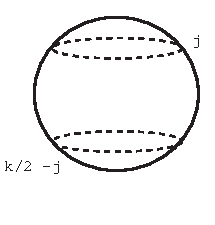
\includegraphics[width=0.28\textwidth,height=0.22\textheight,keepaspectratio]{fig12.pdf}
\caption{由刚性旋转相联系的两张保持对称性的膜。}
\end{figure}


回忆第 5.3 节，我们可以用 \(G_L \times G_R\) 转动我们的膜。有时会出现特殊共轭类可以彼此旋转的情形 \[g_L {\mathcal O}_{\lambda,k} g_R = {\mathcal O}_{\lambda',k} .\] 例如，若 \(G=SU(2)\)，则共轭类 \({\mathcal O}_{j,k}\) 与 \({\mathcal O}_{k/2 - j, k}\) 可以彼此旋转： \[(-1)\cdot {\mathcal O}_{j,k} = {\mathcal O}_{\frac{1}{2} k - j, k}\] 如图 12所示。让我们问：哪些表示以这种方式相关联？

为回答此问题，我们利用紧致连通单连通 Lie 群 \(G\) 的中心与扩张 Dynkin 图的自同构之间的著名关系。例如，若 \(G=SU(N)\)，则 \(Z(G)\cong Z_N\)，而 \(Z_N\) 通过旋转作用在扩张 Dynkin 图上。其次，扩张 Dynkin 图的自同构作用在能级 \(k\) 的可积表示空间 \(P^+_k\) 上。例如对 \(SU(2)\) \[j \to j'= \frac{1}{2} k-j  ,\] 而对 \(\widehat{SU(N)}_k\)，\(Z(G)\) 的生成元按下式作用在 Dynkin 标号上 \[\lambda = (a_1,\dots, a_{N-1}) \to \lambda' = (k-\sum a_i , a_1, \dots, a_{N-2}) .\] 群论的一个优美结果是：若 \(z\in Z(G)\)，则 \[z{\mathcal O}_{\lambda,k} = {\mathcal O}_{z\cdot \lambda ,k}\]

现在我们可用上述公式来确定 D0 荷群的阶。为此先注意，由刚性旋转相联系的两张膜必须具有相同的 D0 荷！另一方面，\(\lambda\) 与 \(z\cdot \lambda\) 具有\emph{不同}的维数，因而具有不同的朴素 D0 荷。因此，我们寻求一个整数 \(d_{k,N}\)，使得 \[d(z\cdot \lambda) = \pm d(\lambda) {\mathrm{mod}} ~ d_{k,N} \qquad \forall z\in Z(G), \lambda\in P^+_k\] 其中符号 \(\pm\) 依赖于 \(z\) 与 \(G\) 的秩，并计及定向（更多细节见 文献）。结果表明，这一条件就确定了 \(d_{k,N}\)： \[d_{k,N}  = {\mathrm gcd}\bigl[\binom{k}{1}, \binom{k}{2},
\dots, \binom{k}{N-1}\bigr].\] 这与 Hopkins 的结果完全一致！（关于其中若干算术的细节见 文献。）

评注：

\begin{itemize}
\item
  \(d_{k,N}\) 对其他紧致单 Lie 群的推广已在 文献 中讨论。
\item
  在我于会议上的报告之后，M. Hopkins 作了一个奇特的评论，我想在此记下。扭曲\emph{等变} K-理论与 \(G\) 的扭曲 K-理论之间有一个简单的数学关系，它与我们刚才给出的物理讨论具有若干相同的要素。若 \(\pi_1(G)\) 无挠，则 文献 的 Künneth 公式提示这两种扭曲 K-理论由下式相联系 \[\mathbb{Z} \otimes_{R(G)} K_{G,H}(G) = K_H(G)\] 这里表示环 \(R(G)\) 应被视为表示簇 \(G/T\) 上（\(T\) 以共轭作用）的函数环。\(R(G)\) 通过表示的维数作用在 \(1\in \mathbb{Z}\) 上，而 \(K_{G,H}(G)\) 是 Verlinde 代数，这要归功于 Freed、Hopkins 与 Teleman 的定理 文献。奇妙的是，从代数几何的角度看，这意味着特殊共轭类（当视为 \(\mathbb{Z}\) 上的簇时）与单位元有交。
\end{itemize}

\subsection{关于陪集模型的评论}\label{ux5173ux4e8eux966aux96c6ux6a21ux578bux7684ux8bc4ux8bba}

上述观点对陪集模型中的膜有潜在有趣的应用。粗略地说，若 \(L\subset G\) 是子群，则 \({\mathcal N}=1\) 超对称陪集模型 \(G/L\) 中的膜应由扭曲等变 K-理论 \(K_{L,H}(G)\) 分类，其中扭曲来自 WZW \(G\)-理论。这类陪集模型中的膜已在许多论文中研究过。作为例子见 文献。对于 \(SU(2)/U(1)\) 模型，文献 中所描述的稳定 \(A\)-膜与扭曲等变 \(K\)-理论完全一致。高秩情形要微妙一些，目前正由 S. Schafer-Nameki 研究 文献。

\SrcRange{37}{37}
\section{结论}\label{ux7ed3ux8bba}

我们在本次报告中的目标并不是建立严格的数学定理，而是要说明：物理如何能为 \(K\)-理论提供某些直观理解，而这些直观理解与该课题更为传统的（并且是严格的！）处理方式相互补充。这类替代性的视角与启发式论证，有时能为研究提示出新的、令人惊讶的方向，有时也能为已知结果提示出简单的启发式解释。上文对 \(SU(N)\) 的扭曲 \(K\)-理论所作的``推导''只是其中一个例子，但还有其他例子。例如，保持对称性的膜恰恰就是那些能下降为 \(G/G\) 规范 WZW 模型中膜的膜。原因在于，规范群通过共轭作用作用于 \(G\)，而只有保持对称性的边界条件才保持这一规范对称性。此外，\(G/G\) WZW 模型是一个拓扑场论，其 Frobenius 代数是 Verlinde 代数。这就为 Freed, Hopkins 和 Teleman 的结果（Freed 2001, 2002；Freed, Hopkins and Teleman 2002）背后的物理提供了一个简单的视角。（这条评注也与（Freed 2001）中的讨论有关。）

最后，我们想提一下若干未来方向作为结束；这些方向可能对数学界来说会是有趣的，并且是由本文所主张的、更为物理的 \(K\)-理论处理方式所提示的。

第一，在时空超对称模型的背景下，一类特殊的边界条件------即所谓的``BPS 态''------可能具有一种有趣的\emph{乘积}结构（Harvey and Moore 1998；Moore 1998）。因此，边界条件的范畴（或某个适当的子范畴）或许也能被赋予张量范畴的结构。

第二，处理 \(D\)-膜的重整化群方法提示了 McKay 对应的一种有趣推广，即推广到轨形奇点的\emph{非 crepant} 环面解（Martinec and Moore 2002）。

最后，II 型弦论中 \(D\)-膜的 \(K\)-理论分类，必定以某种方式与这些理论所具有的 U-对偶对称性相容，也必定以某种方式与 11 维 \(M\)-理论相容。目前人们对这一图景只理解了一些零碎的片段。有可能完整的解决方案会是深刻的，并将具有有趣的数学应用。

\textbf{致谢：} 我要感谢在上面所评述的工作中的各位合作者：E. Diaconescu、D. Kutasov、J. Maldacena、M. Mari\textasciitilde no、N. Saulina、G. Segal、N. Seiberg 和 E. Witten。我从他们那里学到了很多。我还要感谢 N. Andrei、I. Brunner、M. Douglas、D. Freed、D. Friedan、E. Getzler、M. Hopkins、S. Lukyanov、H. Saleur、S. Schafer-Nameki、V. Schomerus、S. Shatashvili、C. Teleman 和 A. Zamolodchikov，感谢他们就这些材料所作的有益讨论与通信。我要感谢 D. Freed 对草稿提出的许多有益意见。最后，我还要感谢 Isaac Newton 研究所在本文写作期间提供的接待，以及 U. Tillmann 邀请我在会议上作报告。本工作部分由 DOE 基金 DE-FG02-96ER40949 资助。



\section*{参考文献}
\noindent{\footnotesize 译注：参考文献保留原文英文条目，编号与原文一致；未逐条中译，以免二次转写失真。}\par\smallskip
\begin{enumerate}[label={[\arabic*]},leftmargin=*,itemsep=2pt]
\item R. Minasian and G. W. Moore, “K-theory and Ramond-Ramond charge,” JHEP 9711, 002 (1997) [arXiv:hep-th/9710230].
\item E. Witten, “D-branes and K-theory,” JHEP 9812, 019 (1998) [arXiv:hep-th/9810188].
\item K. Olsen and R. J. Szabo, “Constructing D-branes from K-theory,” Adv. Theor. Math. Phys. 3, 889 (1999) [arXiv:hep-th/9907140].
\item E. Witten, “Overview of K-theory applied to strings,” Int. J. Mod. Phys. A 16, 693 (2001) [arXiv:hep-th/0007175].
\item D. S. Freed, “K-theory in quantum field theory,” arXiv:math-ph/0206031.
\item R. J. Szabo, “D-branes, tachyons and K-homology,” Mod. Phys. Lett. A 17, 2297 (2002) [arXiv:hep-th/0209210].
\item G. Moore and G. Segal, unpublished. The material is available at http:// on- line.kitp.ucsb.edu/ online/mp01/moore1/ and /moore2, and from lecture notes at the Clay Institute School on Geometry and String Theory, held at the Isaac Newton Institute, Cambridge, UK. April 2002.
\item See lectures by G. Segal at http:// online.kitp.ucsb.edu/ online/geom99, and lecture notes at http:// www.cgtp.duke.edu/ITP99/segal/
\item J. L. Cardy and D. C. Lewellen, “Bulk And Boundary Operators In Conformal Field Theory,” Phys. Lett. B 259, 274 (1991).
\item D. C. Lewellen, “Sewing constraints for conformal field theories on surfaces with boundaries,” Nucl. Phys. B 372, 654 (1992).
\item C. I. Lazaroiu, “On the structure of open-closed topological field theory in two dimen- sions,” Nucl. Phys. B 603, 497 (2001) [arXiv:hep-th/0010269].
\item V. Turaev, “Homotopy field theory in dimension 2 and group-algebras,” arXiv: math.qa/ 9910010.
\item J. Fuchs and C. Schweigert, “Category theory for conformal boundary conditions,” arXiv:math.ct/0106050.
\item J. Fuchs, I. Runkel and C. Schweigert, “Boundaries, defects and Frobenius algebras,” arXiv:hep-th/0302200.
\item I. Bars, “Map of Witten’s * to Moyal’s *,” Phys. Lett. B 517, 436 (2001) [arXiv:hep- th/0106157].
\item M. R. Douglas, H. Liu, G. Moore and B. Zwiebach, “Open string star as a continuous Moyal product,” JHEP 0204, 022 (2002) [arXiv:hep-th/0202087].
\item I. Bars and Y. Matsuo, “Computing in string field theory using the Moyal star prod- uct,” Phys. Rev. D 66, 066003 (2002) [arXiv:hep-th/0204260].
\item I. Bars, “MSFT: Moyal star formulation of string field theory,” arXiv:hep-th/0211238.
\item D. Belov and C. Lovelace, to appear
\item E. Witten, “On background independent open string field theory,” Phys. Rev. D 46, 5467 (1992) [arXiv:hep-th/9208027].
\item D. Friedan, “The Space of Conformal Boundary Conditions for the c = 1 Gaussian Model,” 1993, unpublished.
\item M. R. Gaberdiel and A. Recknagel, “Conformal boundary states for free bosons and fermions,” JHEP 0111, 016 (2001) [arXiv:hep-th/0108238].
\item R. A. Janik, “Exceptional boundary states at c = 1,” Nucl. Phys. B 618, 675 (2001) [arXiv:hep-th/0109021].
\item E. J. Martinec, “Defects, decay, and dissipated states,” arXiv:hep-th/0210231.
\item I. Affleck and A. W. Ludwig, “Universal Noninteger ’Ground State Degeneracy’ In Critical Quantum Systems,” Phys. Rev. Lett. 67, 161 (1991).
\item I. Affleck and A. W. Ludwig, “Exact Conformal Field Theory Results On The Multi- channel Kondo Effect: Single Fermion Green’s Function, Selfenergy And Resistivity,” UBCTP-92-029
\item D. Kutasov, M. Marino and G. W. Moore, “Some exact results on tachyon condensa- tion in string field theory,” JHEP 0010, 045 (2000) [arXiv:hep-th/0009148].
\item D. Kutasov, M. Marino and G. W. Moore, “Remarks on tachyon condensation in superstring field theory,” arXiv:hep-th/0010108.
\item J. A. Harvey, S. Kachru, G. W. Moore and E. Silverstein, “Tension is dimension,” JHEP 0003, 001 (2000) [arXiv:hep-th/9909072].
\item M. Marino, “On the BV formulation of boundary superstring field theory,” JHEP 0106, 059 (2001) [arXiv:hep-th/0103089].
\item V. Niarchos and N. Prezas, “Boundary superstring field theory,” Nucl. Phys. B 619, 51 (2001) [arXiv:hep-th/0103102].
\item A. Connes and D. Kreimer, “Renormalization in quantum field theory and the Riemann-Hilbert problem. II: The beta-function, diffeomorphisms and the renormal- ization group,” Commun. Math. Phys. 216, 215 (2001) [arXiv:hep-th/0003188].
\item A. Connes and D. Kreimer, “Renormalization in quantum field theory and the Riemann-Hilbert problem. I: The Hopf algebra structure of graphs and the main theorem,” Commun. Math. Phys. 210, 249 (2000) [arXiv:hep-th/9912092].
\item E. Witten, “Some computations in background independent off-shell string theory,” Phys. Rev. D 47, 3405 (1993) [arXiv:hep-th/9210065].
\item A. A. Gerasimov and S. L. Shatashvili, “On exact tachyon potential in open string field theory,” JHEP 0010, 034 (2000) [arXiv:hep-th/0009103].
\item A. Sen, “Tachyon condensation on the brane antibrane system,” JHEP 9808, 012 (1998) [arXiv:hep-th/9805170].
\item S. L. Shatashvili, “Comment on the background independent open string theory,” Phys. Lett. B 311, 83 (1993) [arXiv:hep-th/9303143].
\item K. Li and E. Witten, “Role of short distance behavior in off-shell open string field theory,” Phys. Rev. D 48, 853 (1993) [arXiv:hep-th/9303067].
\item S. L. Shatashvili, “On the problems with background independence in string theory,” arXiv:hep-th/9311177.
\item J. A. Harvey, D. Kutasov and E. J. Martinec, “On the relevance of tachyons,” arXiv:hep-th/0003101.
\item A. A. Gerasimov and S. L. Shatashvili, “Stringy Higgs mechanism and the fate of open strings,” JHEP 0101, 019 (2001) [arXiv:hep-th/0011009].
\item P. Baum and R.G. Douglas, “K Homology and Index Theory,” Proc. Symp. Pure Math. 38(1982), 117
\item A. A. Tseytlin, “Born-Infeld action, supersymmetry and string theory,” arXiv:hep- th/9908105.
\item S.K. Donaldson and P.B. Kronheimer, The Geometry of Four-Manifolds, Oxford, 1990
\item K. Hori, A. Iqbal and C. Vafa, “D-branes and mirror symmetry,” arXiv:hep- th/0005247.
\item K. Hori, “Linear models of supersymmetric D-branes,” arXiv:hep-th/0012179.
\item P. Kraus and F. Larsen, “Boundary string field theory of the DD-bar system,” Phys. Rev. D 63, 106004 (2001) [arXiv:hep-th/0012198].
\item T. Takayanagi, S. Terashima and T. Uesugi, “Brane-antibrane action from boundary string field theory,” JHEP 0103, 019 (2001) [arXiv:hep-th/0012210].
\item D. S. Freed, “Dirac charge quantization and generalized differential cohomology,” arXiv:hep-th/0011220.
\item T. Asakawa, S. Sugimoto and S. Terashima, “D-branes, matrix theory and K- homology,” JHEP 0203, 034 (2002) [arXiv:hep-th/0108085].
\item R. J. Szabo, “Superconnections, anomalies and non-BPS brane charges,” J. Geom. Phys. 43, 241 (2002) [arXiv:hep-th/0108043].
\item T. Asakawa, S. Sugimoto and S. Terashima, “Exact description of D-branes via tachyon condensation,” arXiv:hep-th/0212188.
\item V. Periwal, “D-brane charges and K-homology. (Z)),” JHEP 0007, 041 (2000) [arXiv:hep-th/0006223].
\item E. Witten, “Noncommutative tachyons and string field theory,” arXiv:hep-th/0006071.
\item Y. Matsuo, “Topological charges of noncommutative soliton,” Phys. Lett. B 499, 223 (2001) [arXiv:hep-th/0009002].
\item J. A. Harvey and G. W. Moore, “Noncommutative tachyons and K-theory,” J. Math. Phys. 42, 2765 (2001) [arXiv:hep-th/0009030].
\item V. Mathai and I. M. Singer, “Twisted K-homology theory, twisted Ext-theory,” arXiv:hep-th/0012046.
\item M.F. Atiyah, “Global theory of elliptic operators,” Proc. Int. Conf. Func. Anal. and Related Topics, pp. 21-30, Univ. of Tokyo Press, Tokyo, 1970
\item A. Connes, Noncommutative Geometry, Academic Press, 1994
\item E. Witten, “Supersymmetry And Morse Theory,” J. Diff. Geom. 17, 661 (1982).
\item E. Witten, “Global Anomalies In String Theory,” Print-85-0620 (PRINCETON) To appear in Proc. of Argonne Symp. on Geometry, Anomalies and Topology, Argonne, IL, Mar 28-30, 1985
\item G. Segal, “Elliptic cohomology,” Asterisque 161-162(1988) exp. no. 695, 187-201
\item S. Stolz, Contribution to this volume
\item C. Albertsson, U. Lindstrom and M. Zabzine, “N = 1 supersymmetric sigma model with boundaries. I,” arXiv:hep-th/0111161.
\item C. Albertsson, U. Lindstrom and M. Zabzine, “N = 1 supersymmetric sigma model with boundaries. II,” arXiv:hep-th/0202069.
\item U. Lindstrom, M. Rocek and P. van Nieuwenhuizen, “Consistent boundary conditions for open strings,” arXiv:hep-th/0211266.
\item A. Jaffe, A. Lesniewski and J. Weitsman, “Index Of A Family Of Dirac Operators On Loop Space,” Commun. Math. Phys. 112, 75 (1987).
\item A. Jaffe, A. Lesniewski and K. Osterwalder, “Quantum K Theory. 1. The Chern Character,” Commun. Math. Phys. 118, 1 (1988).
\item K. Ernst, P. Feng, A. Jaffe and A. Lesniewski, “Quantum K Theory. 2. Homotopy Invariance Of The Chern Character,” HUTMP-88/B-228
\item N. Seiberg and E. Witten, “String theory and noncommutative geometry,” JHEP 9909, 032 (1999) [arXiv:hep-th/9908142].
\item J. M. Maldacena, G. W. Moore and N. Seiberg, “D-brane instantons and K-theory charges,” JHEP 0111, 062 (2001) [arXiv:hep-th/0108100].
\item A. Kapustin, “D-branes in a topologically nontrivial B-field,” Adv. Theor. Math. Phys. 4, 127 (2000) [arXiv:hep-th/9909089].
\item P. Bouwknegt and V. Mathai, “D-branes, B-fields and twisted K-theory,” JHEP 0003, 007 (2000) [arXiv:hep-th/0002023].
\item P. Bouwknegt, A. L. Carey, V. Mathai, M. K. Murray and D. Stevenson, “Twisted K-theory and K-theory of bundle gerbes,” Commun. Math. Phys. 228, 17 (2002) [arXiv:hep-th/0106194].
\item K. Gawedzki and N. Reis, “WZW branes and gerbes,” arXiv:hep-th/0205233.
\item J. Evslin and U. Varadarajan, “K-theory and S-duality: Starting over from square 3,” arXiv:hep-th/0112084.
\item J. Evslin, “Twisted K-theory from monodromies,” arXiv:hep-th/0302081.
\item D. S. Freed and E. Witten, “Anomalies in string theory with D-branes,” arXiv:hep- th/9907189.
\item E. Witten, “Baryons and branes in anti de Sitter space,” JHEP 9807, 006 (1998) [arXiv:hep-th/9805112].
\item D. E. Diaconescu, G. W. Moore and E. Witten, “E(8) gauge theory, and a derivation of K-theory from M-theory,” arXiv:hep-th/0005090.
\item A. Alekseev and V. Schomerus, “RR charges of D2-branes in the WZW model,” arXiv:hep-th/0007096.
\item S. Fredenhagen and V. Schomerus, “Branes on group manifolds, gluon condensates, and twisted K-theory,” JHEP 0104, 007 (2001) [arXiv:hep-th/0012164].
\item S. Stanciu, “An illustrated guide to D-branes in SU(3),” arXiv:hep-th/0111221.
\item V. Schomerus, “Lectures on branes in curved backgrounds,” Class. Quant. Grav. 19, 5781 (2002) [arXiv:hep-th/0209241].
\item C. Schweigert, J. Fuchs and J. Walcher, “Conformal field theory, boundary conditions and applications to string theory,” arXiv:hep-th/0011109.
\item K. Gawedzki, “Boundary WZW, G/H, G/G and CS theories,” Annales Henri Poincare 3, 847 (2002) [arXiv:hep-th/0108044].
\item A. Pressley and G. Segal, Loop Groups, Oxford, 1986
\item G. Felder, J. Frohlich, J. Fuchs and C. Schweigert, “The geometry of WZW branes,” J. Geom. Phys. 34, 162 (2000) [arXiv:hep-th/9909030].
\item J. M. Maldacena, G. W. Moore and N. Seiberg, “Geometrical interpretation of D- branes in gauged WZW models,” JHEP 0107, 046 (2001) [arXiv:hep-th/0105038].
\item I. R. Klebanov and L. Thorlacius, “The Size of p-Branes,” Phys. Lett. B 371, 51 (1996) [arXiv:hep-th/9510200].
\item M. R. Douglas, “Two lectures on D-geometry and noncommutative geometry,” arXiv:hep-th/9901146.
\item M. R. Douglas, “D-branes on Calabi-Yau manifolds,” arXiv:math.ag/0009209.
\item M. R. Douglas, “D-branes in curved space,” Adv. Theor. Math. Phys. 1, 198 (1998) [arXiv:hep-th/9703056].
\item C. Bachas, M. R. Douglas and C. Schweigert, “Flux stabilization of D-branes,” JHEP 0005, 048 (2000) [arXiv:hep-th/0003037].
\item J. Pawelczyk, “SU(2) WZW D-branes and their noncommutative geometry from DBI action,” JHEP 0008, 006 (2000) [arXiv:hep-th/0003057].
\item P. Bordalo, S. Ribault and C. Schweigert, “Flux stabilization in compact groups,” JHEP 0110, 036 (2001) [arXiv:hep-th/0108201].
\item J. M. Maldacena, G. W. Moore and N. Seiberg, “D-brane charges in five-brane back- grounds,” JHEP 0110, 005 (2001) [arXiv:hep-th/0108152].
\item Y. Hikida, M. Nozaki and Y. Sugawara, “Formation of spherical D2-brane from mul- tiple D0-branes,” Nucl. Phys. B 617, 117 (2001) [arXiv:hep-th/0101211].
\item D. Friedan, Z. Qiu, and S.H. Shenker, Phys. Lett. 151B(1985)37
\item P. di Vecchia, V.G. Knizhnik, J.L. Petersen, and P. Rossi, Nucl. Phys. B253(1985)
\item V.G. Kac and I.T. Todorov, Comm. Math. Phys. 102(1985)337
\item V. V. Bazhanov, S. L. Lukyanov and A. B. Zamolodchikov, “Integrable structure of conformal field theory, quantum KdV theory and thermodynamic Bethe ansatz,” Commun. Math. Phys. 177, 381 (1996) [arXiv:hep-th/9412229].
\item V. V. Bazhanov, S. L. Lukyanov and A. B. Zamolodchikov, “Integrable Structure of Conformal Field Theory II. Q-operator and DDV equation,” Commun. Math. Phys. 190, 247 (1997) [arXiv:hep-th/9604044].
\item V. V. Bazhanov, S. L. Lukyanov and A. B. Zamolodchikov, “Integrable structure of conformal field theory. III: The Yang-Baxter relation,” Commun. Math. Phys. 200, 297 (1999) [arXiv:hep-th/9805008].
\item N. Andrei, “Integrable Models in Condensed Matter Physics,” cond-mat/9408101
\item P. Fendley, F. Lesage and H. Saleur, “A unified framework for the Kondo problem and for an impurity in a Luttinger liquid,” arXiv:cond-mat/9510055.
\item F. Lesage, H. Saleur and P. Simonetti, “Boundary flows in minimal models,” Phys. Lett. B 427, 85 (1998) [arXiv:hep-th/9802061].
\item J. Mickelsson, “Gerbes, (twisted) K-theory, and the supersymmetric WZW model,” arXiv:hep-th/0206139.
\item D. Freed, M. Hopkins, and C. Teleman, presented by D. Freed, at “Elliptic Cohomology and Chromatic Phenomena,” Dec. 2002, Isaac Newton Institute.
\item I. Affleck, “Conformal Field Theory Approach to the Kondo Effect,” Acta Phys. Polon. B 26, 1869 (1995) [arXiv:cond-mat/9512099].
\item R. C. Myers, “Dielectric-branes,” JHEP 9912, 022 (1999) [arXiv:hep-th/9910053].
\item P. Bouwknegt, P. Dawson and D. Ridout, “D-branes on group manifolds and fusion rings,” JHEP 0212, 065 (2002) [arXiv:hep-th/0210302].
\item V.P. Snaith, “On the Kunneth formula spectral sequence in equivariant K-theory,” Proc. Camb. Phil. Soc. 72(1972)167
\item L. Hodgkin, “The equivariant Kunneth theorem in K-theory,” Springer Lect. Notes in Math, 496, pp. 1-101, 1975
\item D. S. Freed, “The Verlinde algebra is twisted equivariant K-theory,” arXiv:math.rt/0101038.
\item D. S. Freed, “Twisted K-theory and loop groups,” arXiv:math.at/0206237.
\item D.S. Freed, M.J. Hopkins, and C. Teleman, “Twisted equivariant K-theory with com- plex coefficients,” math.AT/0206257
\item W. Lerche and J. Walcher, “Boundary rings and N = 2 coset models,” Nucl. Phys. B 625, 97 (2002) [arXiv:hep-th/0011107].
\item F. Falceto and K. Gawedzki, “Boundary G/G theory and topological Poisson-Lie sigma model,” Lett. Math. Phys. 59, 61 (2002) [arXiv:hep-th/0108206].
\item S. Fredenhagen and V. Schomerus, “D-branes in coset models,” JHEP 0202, 005 (2002) [arXiv:hep-th/0111189].
\item S. Fredenhagen and V. Schomerus, “On boundary RG-flows in coset conformal field theories,” arXiv:hep-th/0205011.
\item S. Fredenhagen, “Organizing boundary RG flows,” arXiv:hep-th/0301229.
\item S. Schafer-Nameki, to appear.
\item J. A. Harvey and G. W. Moore, “On the algebras of BPS states,” Commun. Math. Phys. 197, 489 (1998) [arXiv:hep-th/9609017].
\item G. W. Moore, “String duality, automorphic forms, and generalized Kac-Moody alge- bras,” Nucl. Phys. Proc. Suppl. 67, 56 (1998) [arXiv:hep-th/9710198].
\item E. J. Martinec and G. Moore, “On decay of K-theory,” arXiv:hep-th/0212059.
\end{enumerate}

\end{document}
